\documentclass[12pt,a4paper]{article}

% ---------------------------------------------------------------- packages
\usepackage[T1]{fontenc}
\usepackage{lmodern}
\usepackage[a4paper,top=2.6cm,bottom=2.8cm,left=2.5cm,right=2.5cm,headheight=15pt]{geometry}
\usepackage{amsmath,amssymb}
\usepackage{graphicx}
\usepackage{booktabs,array,multirow,tabularx,longtable}
\usepackage{float}
\usepackage[font=small,labelfont=bf]{caption}
\usepackage{enumitem}
\usepackage{xcolor}
\usepackage{fancyhdr}
\usepackage{tikz}
\usetikzlibrary{positioning,arrows.meta,shapes.geometric,calc,fit}
\usepackage{algorithm}
\usepackage{algpseudocode}
\usepackage{listings}
\usepackage{setspace}
\usepackage{microtype}
\usepackage[hidelinks]{hyperref}

% ---------------------------------------------------------------- project details (edit here)
\newcommand{\ProjectTitle}{Parkinson's Disease Severity Prediction from Voice Recordings using Support Vector Regression Optimised with Cuckoo Search}
\newcommand{\RepoURL}{https://github.com/Aniketh2435/Parkinsons-Cuckoo-SVR}
\newcommand{\GuideName}{Prof. Manoj Kumar}
\newcommand{\GuideDesignation}{Assistant Professor}
\newcommand{\AcademicYear}{AY 2026--2027}

% ---------------------------------------------------------------- page style: rounded border + footer
\definecolor{bmsblue}{RGB}{20,40,220}
\definecolor{titlered}{RGB}{220,20,20}
\newcommand{\pageborder}{%
  \begin{tikzpicture}[remember picture,overlay]
    \draw[line width=2.2pt,color=black!55,rounded corners=10pt]
      ($(current page.north west)+(0.45cm,-0.45cm)$) rectangle ($(current page.south east)+(-0.45cm,0.45cm)$);
  \end{tikzpicture}}
\pagestyle{fancy}
\fancyhf{}
\renewcommand{\headrulewidth}{0pt}
\fancyhead[C]{\pageborder}
\fancyfoot[C]{Department of CSE (Data Science)}
\fancyfoot[R]{\thepage}
\fancypagestyle{coverpage}{\fancyhf{}\fancyhead[C]{\pageborder}}
\fancypagestyle{plain}{\fancyhf{}\fancyhead[C]{\pageborder}\fancyfoot[C]{Department of CSE (Data Science)}\fancyfoot[R]{\thepage}}

\setstretch{1.25}
\setlength{\parskip}{4pt}
\setlist{itemsep=2pt,topsep=4pt}
\numberwithin{equation}{section}
\numberwithin{table}{section}
\numberwithin{figure}{section}

\lstset{basicstyle=\ttfamily\scriptsize,breaklines=true,frame=single,numbers=left,numberstyle=\tiny\color{gray},
  keywordstyle=\color{blue!70!black}\bfseries,commentstyle=\color{green!45!black},stringstyle=\color{red!60!black},
  showstringspaces=false,columns=fullflexible,language=Python}

\newcommand{\RMSE}{\mathrm{RMSE}}

\begin{document}

% ================================================================= COVER
\begin{titlepage}
\thispagestyle{coverpage}
\centering\setstretch{1.0}
{\color{bmsblue}\Large\bfseries B.M.S. COLLEGE OF ENGINEERING\par}
\vspace{0.25cm}
{\large\bfseries (Autonomous College under VTU)\par}
\vspace{0.15cm}
{\large\bfseries Bull Temple Road, Basavangudi, Bangalore - 560019\par}
\vspace{0.45cm}

\includegraphics[width=4.2cm]{figures/bmsce_logo.png}\par
\vspace{0.45cm}
{\itshape Bio Inspired Algorithms AAT on\par}
\vspace{0.3cm}
{\color{titlered}\large\bfseries Parkinson's Disease Severity Prediction from Voice Recordings using Support Vector Regression Optimised with Cuckoo Search\par}
\vspace{0.4cm}
{\itshape in fulfillment of the requirements for the award of degree\par}
\vspace{0.3cm}
{\bfseries BACHELOR OF ENGINEERING\par}
\vspace{0.15cm}
{\itshape in\par}
\vspace{0.15cm}
{\bfseries Computer Science \& Engineering (Data Science)\par}
\vspace{0.15cm}
{\itshape by\par}
\vspace{0.2cm}
{\bfseries Abhijith M Reddy (1BM23CD003)\par}
{\bfseries Aniketh S Nadig (1BM23CD006)\par}
{\bfseries Mayur M (1BM23CD037)\par}
{\bfseries S Sanjay (1BM23CD053)\par}
{\bfseries Tanush V Gowda (1BM23CD064)\par}
\vspace{0.35cm}
{\bfseries Under the Guidance of\par}
\vspace{0.15cm}
{\bfseries \GuideName\par}
{\GuideDesignation\par}
\vspace{0.35cm}
{\bfseries Department of CSE (Data Science),\par}
{\bfseries B.M.S. College of Engineering\par}
\vspace{0.3cm}
{\bfseries \AcademicYear\par}
\end{titlepage}

% ================================================================= CERTIFICATE
\setcounter{page}{1}
\begingroup\setstretch{1.0}
\begin{center}
{\color{bmsblue}\Large\bfseries B.M.S. COLLEGE OF ENGINEERING\par}
\vspace{0.2cm}
{\large\bfseries (Autonomous College under VTU)\par}
\vspace{0.1cm}
{\large\bfseries Bull Temple Road, Basavangudi, Bangalore - 560019\par}
\vspace{0.25cm}

\includegraphics[width=2.6cm]{figures/bmsce_logo.png}\par
\vspace{0.25cm}
{\bfseries Department of Computer Science and Engineering\par (Data Science)\par}
\vspace{0.1cm}
{\Large\bfseries\underline{CERTIFICATE}\par}
\end{center}

\noindent This is to certify that the project entitled \textbf{``\ProjectTitle''} is a bona fide work carried out by the following students for the course Bio Inspired Algorithms (Course Code: \textbf{23DS7BSBIO}). It is certified that all corrections and suggestions indicated during the internal assessments have been incorporated in the final report submitted to the departmental library. The project report has been approved as it meets the academic requirements prescribed for the Bachelor of Engineering Degree in respect of project work.

\begin{center}
\textbf{\underline{Candidate details}}\\[0.25cm]
\renewcommand{\arraystretch}{1.3}
\begin{tabular}{|c|l|c|p{4.0cm}|}
\hline
\textbf{SL. NO.} & \textbf{Student Name} & \textbf{USN} & \textbf{Student's Signature}\\ \hline
1 & Abhijith M Reddy & 1BM23CD003 & \\ \hline
2 & Aniketh S Nadig & 1BM23CD006 & \\ \hline
3 & Mayur M & 1BM23CD037 & \\ \hline
4 & S Sanjay & 1BM23CD053 & \\ \hline
5 & Tanush V Gowda & 1BM23CD064 & \\ \hline
\end{tabular}
\end{center}

\vspace{0.3cm}
\noindent\begin{minipage}[t]{0.5\textwidth}
\textbf{Signature of the Guide}\\[0.25cm]
\textbf{\GuideName}\\
\GuideDesignation
\end{minipage}%
\begin{minipage}[t]{0.5\textwidth}
\raggedleft
\textbf{Signature of the HOD}\\[0.25cm]
\textbf{Dr. Shambhavi B R}\\
Professor \& HOD
\end{minipage}

\vspace{0.3cm}
\begin{center}\textbf{Examiners}\end{center}
\noindent\textbf{Name of Examiner}\hfill\textbf{Signature of the Examiner}\\[0.4cm]
\textbf{1.}\hfill\rule{4.5cm}{0.4pt}\\[0.4cm]
\textbf{2.}\hfill\rule{4.5cm}{0.4pt}
\endgroup

\newpage
% ================================================================= ACKNOWLEDGEMENTS
\begin{center}{\large\bfseries Acknowledgements}\end{center}
\addcontentsline{toc}{section}{Acknowledgements}

We would take this opportunity to express our heart-felt gratitude to \textbf{Dr. B. S. Ragini Narayan}, \textit{Chairperson}, Donor Trustee, Member Secretary \& Chairperson, BMSET, \textbf{Dr. P. Dayananda Pai}, \textit{Member Life Trustee}, BMSET and \textbf{Dr. Bheemsha Arya}, \textit{Principal}, B.M.S. College of Engineering for providing the necessary infrastructure to complete this Alternative Assessment.

We wish to express our deepest gratitude to \textbf{Dr. Shambhavi B R}, Head of the Department, Computer Science and Engineering (Data Science), and our Project Guide \textbf{\GuideName} for their constant support.

A warm thanks to all the faculty of the Department of Computer Science and Engineering (Data Science), who have helped us with their views and encouraging ideas.

\newpage
\tableofcontents
\newpage
\listoffigures
\addcontentsline{toc}{section}{List of Figures}
\listoftables
\addcontentsline{toc}{section}{List of Tables}
\newpage

% ================================================================= ABSTRACT
\begin{center}{\large\bfseries Abstract}\end{center}
\addcontentsline{toc}{section}{Abstract}

Parkinson's disease (PD) is a progressive neurodegenerative disorder whose severity is tracked by clinicians with the Unified Parkinson's Disease Rating Scale (UPDRS). Measuring UPDRS requires a clinic visit, while voice impairment appears early in PD and can be recorded at home. This project predicts the clinician-rated \emph{motor UPDRS} score from biomedical voice measurements using the Oxford Parkinson's Disease Telemonitoring dataset (5,875 recordings from 42 patients, 18 input features).

An RBF-kernel Support Vector Regressor (SVR) is used as the predictive model. Its accuracy depends strongly on three hyperparameters ($C$, $\gamma$, $\varepsilon$) and on which input features it receives, and the library defaults give only $R^2 = 0.50$. We implement \textbf{Cuckoo Search} (Yang \& Deb, 2009) from scratch---Lévy flights generated with Mantegna's algorithm, greedy nest replacement, nest abandonment, elitism and a warm start---and use it to tune the three hyperparameters \emph{and} select the feature subset jointly, encoding each candidate as a 21-dimensional nest. Fitness is the 3-fold cross-validated RMSE on the training set; the test set is never seen during the search.

The implementation is first validated on four standard benchmark functions, where it outperforms Random Search on every function (by up to five orders of magnitude) and exposes (and we correct) a population-collapse bug in an earlier version. On the held-out test set the Cuckoo-optimised SVR reduces RMSE from 5.672 to \textbf{4.347 (23.4\% lower)}, MAE by \textbf{30.5\%}, and raises $R^2$ from 0.496 to \textbf{0.704} while using only 9 of the 18 features. Over 10 independent runs it beats the default SVR in 10/10 runs (Wilcoxon $p = 0.001$) and a same-budget Random Search in 8/10 runs with a mean test RMSE of $4.356 \pm 0.042$ versus $4.596 \pm 0.186$ (Wilcoxon $p = 0.005$). All code, logs and figures are saved in an executed Jupyter notebook for reproducibility.

\vspace{0.3cm}
\noindent\textbf{Keywords:} Cuckoo Search, Lévy flight, Support Vector Regression, hyperparameter optimisation, feature selection, Parkinson's disease, telemonitoring, UPDRS.

\newpage

% ================================================================= 1 INTRODUCTION
\section{Introduction}

\subsection{Background and Motivation}
Parkinson's disease is the second most common neurodegenerative disorder after Alzheimer's disease, affecting millions of people worldwide, mostly over the age of 60 \cite{poewe2017}. Its motor symptoms---tremor, rigidity, slowness of movement and postural instability---worsen over years, and treatment has to be adjusted as the disease progresses. Clinicians measure severity with the Unified Parkinson's Disease Rating Scale (UPDRS) \cite{goetz2008}; its motor section is scored by a trained examiner in a physical examination.

Tracking progression this way has practical problems:
\begin{itemize}
  \item Patients must travel to a clinic, which is difficult for elderly people with movement disorders.
  \item Assessments are infrequent (often months apart), so short-term changes are missed.
  \item Scoring depends on the examiner and requires specialist time.
\end{itemize}

Speech is affected in the majority of PD patients, often early: the voice becomes quieter, breathier and less stable (dysphonia). These changes can be quantified from a short sustained-vowel recording made on a phone or a home device \cite{little2009}. If a model can map such voice measurements to the UPDRS score accurately, disease progression can be monitored remotely, frequently and cheaply \cite{tsanas2010}.

\subsection{Problem Statement}
Given 16 dysphonia measures extracted from a voice recording, plus the patient's age and sex, predict the clinician's motor UPDRS score (a continuous value between about 5 and 40 in this dataset). This is a non-linear regression problem with correlated, skewed inputs.

A Support Vector Regressor with an RBF kernel suits such problems, but its accuracy is highly sensitive to:
\begin{itemize}
  \item the regularisation parameter $C$, the kernel width $\gamma$ and the tube width $\varepsilon$, which interact non-linearly and span several orders of magnitude;
  \item the input features: several voice measures are near-duplicates of one another, and irrelevant inputs distort RBF distances.
\end{itemize}
Choosing these by hand or keeping library defaults gives poor results (default SVR: $R^2 = 0.50$). The joint space of three continuous hyperparameters and $2^{18}$ feature subsets is mixed, non-convex and has no gradient, which makes it a natural target for a nature-inspired metaheuristic.

\subsection{Objectives}
\begin{enumerate}
  \item Prepare the Parkinson's telemonitoring dataset: clean it, transform skewed features and split it into training and test sets.
  \item Build baseline models without optimisation (mean predictor, linear regression, default SVR).
  \item Implement Cuckoo Search from scratch, with all its operators, and validate it on standard benchmark functions.
  \item Apply Cuckoo Search to jointly tune the SVR hyperparameters and select the input features.
  \item Compare the optimised model against the baselines and against Random Search with the same evaluation budget, using RMSE, MAE, $R^2$ and MAPE, convergence curves and learning curves.
  \item Test whether the improvements are robust across independent runs, using non-parametric statistical tests.
\end{enumerate}

\subsection{Contributions}
\begin{itemize}
  \item A from-scratch, documented Cuckoo Search implementation for a mixed continuous--binary search space (log-scaled hyperparameters + threshold-transfer feature bits).
  \item Joint hyperparameter tuning and feature selection for SVR, reducing test RMSE by 23.4\% and halving the number of features (18 $\rightarrow$ 9).
  \item A benchmark-function validation and ablation study showing why greedy per-nest replacement matters: the variant that replaces a random nest collapses the population and stalls.
  \item A fair comparison against Random Search (same budget, same fitness function) over 10 seeds, with Wilcoxon signed-rank tests.
  \item A fully reproducible pipeline: seeded code, an executed notebook with all logs and timestamps, and every figure and metric saved to disk.
\end{itemize}

\subsection{Report Organisation}
Section~\ref{sec:lit} reviews related work. Section~\ref{sec:theory} gives the theory behind SVR, feature selection, Lévy flights and the evaluation metrics. Section~\ref{sec:nia} studies nature-inspired algorithms in detail and justifies the choice of Cuckoo Search. Section~\ref{sec:method} describes the methodology and implementation, and Section~\ref{sec:setup} the experimental setup. Section~\ref{sec:results} presents and discusses the results. Sections~\ref{sec:conclusion} and~\ref{sec:future} conclude and outline future work.

% ================================================================= 2 LITERATURE REVIEW
\section{Literature Review}\label{sec:lit}

\subsection{Voice as a Biomarker for Parkinson's Disease}
Little et al.\ \cite{little2009} showed that dysphonia measures computed from sustained vowel phonations---including classical jitter and shimmer and newer non-linear measures such as RPDE, DFA and PPE---can separate people with PD from healthy controls. Sakar et al.\ \cite{sakar2013} collected a further PD speech dataset with several types of recordings and confirmed that sustained vowels carry the most discriminative information. These studies established voice as a cheap, non-invasive biomarker.

\subsection{Machine Learning for UPDRS Prediction}
Tsanas et al.\ \cite{tsanas2010} introduced the telemonitoring dataset used in this project: recordings captured automatically in patients' homes over a six-month trial. They mapped dysphonia measures to motor and total UPDRS with linear regression and non-linear methods (including CART), and found that non-linear models were clearly more accurate, supporting remote monitoring. Eskidere et al.\ \cite{eskidere2012} compared several regression methods on the same data, including support vector machines and least-squares SVMs, and again reported that kernel methods outperform linear ones. These works motivate a non-linear kernel regressor, but they tune hyperparameters by hand or by grid search.

\subsection{Support Vector Regression and Its Hyperparameters}
SVR \cite{vapnik1995,smola2004} fits a function that keeps most training points inside an $\varepsilon$-wide tube while staying as flat as possible. With an RBF kernel its behaviour is governed by $C$ (penalty on points outside the tube), $\gamma$ (kernel width) and $\varepsilon$. Hsu et al.\ \cite{hsu2003} recommend searching $C$ and $\gamma$ on exponentially spaced grids because good values vary over orders of magnitude, an approach we follow by searching on a $\log_{10}$ scale.

\subsection{Hyperparameter Optimisation Methods}
Grid search scales exponentially with the number of parameters. Bergstra and Bengio \cite{bergstra2012} showed that random search is more efficient than grid search when only a few parameters matter, which makes it a strong, simple baseline. Bayesian optimisation \cite{snoek2012} builds a surrogate model of the objective but handles high-dimensional binary inputs such as feature masks poorly. Population-based metaheuristics make no assumptions about the objective and treat continuous and binary variables in the same framework.

\subsection{Nature-Inspired Tuning of SVMs with Feature Selection}
Huang and Wang \cite{huang2006} used a Genetic Algorithm (GA) to optimise SVM parameters and the feature subset \emph{simultaneously}, and showed that doing both together gives better accuracy with fewer features than doing either alone. Lin et al.\ \cite{lin2008} achieved the same with Particle Swarm Optimisation (PSO), using a continuous-to-binary mapping for the feature part. Our encoding follows this joint ``hyperparameters + feature mask'' design.

\subsection{Cuckoo Search and Its Applications}
Cuckoo Search was proposed by Yang and Deb \cite{yang2009} and applied to engineering design problems in \cite{yang2010eng}, where it matched or beat GA and PSO with fewer tunable parameters. Its key ingredient, the Lévy flight, gives occasional long jumps that help the search escape local optima. Rodrigues et al.\ \cite{rodrigues2013} proposed a binary Cuckoo Search for feature selection, using a transfer function to map continuous positions to bits; transfer functions for binary swarm algorithms are studied by Mirjalili and Lewis \cite{mirjalili2013}.

\subsection{Research Gap}
\begin{itemize}
  \item Prior UPDRS-prediction work tunes models manually or by grid search; nature-inspired joint tuning and feature selection of SVR for this task is rarely reported.
  \item Many metaheuristic studies compare only against untuned baselines and not against Random Search with the \emph{same} budget, so it is unclear whether the bio-inspired operators themselves help.
  \item Results are often from a single run; robustness across seeds and statistical significance are seldom tested.
\end{itemize}
This project addresses all three points.

% ================================================================= 3 THEORY
\section{Theoretical Background}\label{sec:theory}

\subsection{Problem Formulation}
Let $\{(\mathbf{x}_i, y_i)\}_{i=1}^{n}$ be the training data, with $\mathbf{x}_i \in \mathbb{R}^{18}$ the voice and demographic features of recording $i$ and $y_i$ its motor UPDRS score. We learn $\hat{y} = f(\mathbf{x}; \boldsymbol{\theta}, \mathbf{m})$, where $\boldsymbol{\theta} = (C, \gamma, \varepsilon)$ are the SVR hyperparameters and $\mathbf{m} \in \{0,1\}^{18}$ is a feature mask. The optimisation problem is
\begin{equation}
  (\boldsymbol{\theta}^*, \mathbf{m}^*) = \arg\min_{\boldsymbol{\theta},\, \mathbf{m}} \; \mathrm{CV\text{-}RMSE}\big(f(\,\cdot\,; \boldsymbol{\theta}, \mathbf{m})\big).
\end{equation}

\subsection{Support Vector Regression}
For a feature map $\phi$, $\varepsilon$-SVR \cite{smola2004} solves
\begin{align}
  \min_{\mathbf{w}, b, \xi, \xi^*} \quad & \tfrac{1}{2}\|\mathbf{w}\|^2 + C \sum_{i=1}^{n} (\xi_i + \xi_i^*) \\
  \text{s.t.} \quad & y_i - \mathbf{w}^\top\phi(\mathbf{x}_i) - b \le \varepsilon + \xi_i, \\
  & \mathbf{w}^\top\phi(\mathbf{x}_i) + b - y_i \le \varepsilon + \xi_i^*, \qquad \xi_i, \xi_i^* \ge 0 .
\end{align}
Errors smaller than $\varepsilon$ are ignored; larger ones are penalised linearly with weight $C$. The dual solution gives
\begin{equation}
  f(\mathbf{x}) = \sum_{i=1}^{n} (\alpha_i - \alpha_i^*)\, K(\mathbf{x}_i, \mathbf{x}) + b,
\end{equation}
where only the support vectors (points on or outside the tube) have non-zero $\alpha_i - \alpha_i^*$.

\subsection{The RBF Kernel and the Role of Each Hyperparameter}
The radial basis function kernel is
\begin{equation}
  K(\mathbf{x}, \mathbf{x}') = \exp\!\big(-\gamma \, \|\mathbf{x} - \mathbf{x}'\|^2\big).
\end{equation}
\begin{itemize}
  \item \textbf{$\gamma$} sets the reach of each training point: a small $\gamma$ gives a smooth, almost linear function (underfitting); a large $\gamma$ gives a very wiggly function (overfitting).
  \item \textbf{$C$} trades flatness against training error: a large $C$ fits the training data closely.
  \item \textbf{$\varepsilon$} sets the width of the insensitive tube and so the number of support vectors.
\end{itemize}
Because $\gamma$ acts on squared distances, irrelevant or redundant features change the distances between all points. This is why feature selection and hyperparameters must be chosen together.

\subsection{Feature Selection as a Wrapper Problem}
In a \emph{wrapper} approach the quality of a feature subset is measured by the cross-validated error of the model trained on it. Exhaustive search over $2^{18} = 262{,}144$ subsets, each combined with continuous hyperparameters, is infeasible, so a metaheuristic is used. Continuous positions are mapped to bits with a threshold transfer function \cite{mirjalili2013}:
\begin{equation}
  m_j = \begin{cases} 1 & \text{if } x_{3+j} > 0.5 \\ 0 & \text{otherwise.}\end{cases}
\end{equation}

\subsection{Lévy Flights}
A Lévy flight is a random walk whose step lengths follow a heavy-tailed distribution,
\begin{equation}
  L(s) \sim |s|^{-1-\beta}, \qquad 0 < \beta \le 2 .
\end{equation}
Most steps are short, but occasional steps are very long. Such patterns have been observed in the foraging paths of many animals \cite{yang2010book}. For optimisation this gives a natural balance: short steps refine the current solution (exploitation) and rare long jumps explore distant regions (exploration). Lévy steps are generated with \textbf{Mantegna's algorithm} \cite{mantegna1994}:
\begin{equation}
  s = \frac{u}{|v|^{1/\beta}}, \qquad u \sim \mathcal{N}(0, \sigma_u^2), \quad v \sim \mathcal{N}(0, 1),
\end{equation}
\begin{equation}
  \sigma_u = \left[ \frac{\Gamma(1+\beta)\, \sin(\pi\beta/2)}{\Gamma\!\big(\frac{1+\beta}{2}\big)\, \beta\, 2^{(\beta-1)/2}} \right]^{1/\beta}.
\end{equation}
For $\beta = 1.5$ (used here), $\sigma_u \approx 0.6966$.

\subsection{Evaluation Metrics}
For $n$ test recordings with true scores $y_i$, predictions $\hat{y}_i$ and mean $\bar{y}$:
\begin{align}
  \RMSE &= \sqrt{\frac{1}{n}\sum_{i=1}^{n} (y_i - \hat{y}_i)^2} \\
  \mathrm{MAE} &= \frac{1}{n}\sum_{i=1}^{n} |y_i - \hat{y}_i| \\
  R^2 &= 1 - \frac{\sum_{i}(y_i - \hat{y}_i)^2}{\sum_{i}(y_i - \bar{y})^2} \\
  \mathrm{MAPE} &= \frac{100\%}{n}\sum_{i=1}^{n} \left| \frac{y_i - \hat{y}_i}{y_i} \right|
\end{align}
RMSE and MAE are in UPDRS points. RMSE penalises large errors more strongly. $R^2$ is the fraction of variance explained (0 for a constant mean prediction). MAPE is well defined because UPDRS is always positive.

\subsection{Wilcoxon Signed-Rank Test}
To compare two methods over $k$ paired runs, the Wilcoxon signed-rank test \cite{wilcoxon1945} ranks the absolute differences $|d_i|$ and sums the ranks of the positive ones:
\begin{equation}
  W = \sum_{i=1}^{k} \mathbb{1}[d_i > 0] \cdot R_i .
\end{equation}
It does not assume normally distributed differences, which suits stochastic optimisers. We use the one-sided alternative ``Cuckoo Search has lower test RMSE''.

% ================================================================= 4 NIA STUDY
\section{Nature-Inspired Algorithms: Detailed Study}\label{sec:nia}

\subsection{Overview of Nature-Inspired Optimisation}
Nature-inspired algorithms imitate biological, physical or social processes to search large spaces without gradients. They maintain one or more candidate solutions and improve them with stochastic operators that balance \emph{exploration} (visiting new regions) and \emph{exploitation} (refining good regions). Advantages for hyperparameter tuning:
\begin{itemize}
  \item no gradient or smoothness assumptions---the fitness can be a cross-validation score;
  \item continuous and discrete (binary) variables can be searched together;
  \item population-based search is robust to local optima and to noise in the fitness;
  \item candidate solutions in one generation can be evaluated in parallel.
\end{itemize}
By the No Free Lunch theorem \cite{wolpert1997} no algorithm is best on all problems, so an algorithm must be chosen for the structure of the problem and validated empirically.

\subsection{Cuckoo Search: In-Depth Analysis}

\paragraph{Biological inspiration.} Some cuckoo species practise \emph{brood parasitism}: they lay eggs in the nests of other bird species. If the host bird discovers the foreign egg, it throws it out or abandons the nest and builds a new one elsewhere. Cuckoo eggs that look like the host's own eggs are more likely to survive, so over generations the cuckoos' eggs become better ``solutions''.

\paragraph{Idealised rules.} Yang and Deb \cite{yang2009} turned this behaviour into three rules:
\begin{enumerate}
  \item Each cuckoo lays one egg at a time and dumps it in a randomly chosen nest; the egg is a new candidate solution generated by a Lévy flight.
  \item The best nests with the highest-quality eggs are carried over to the next generation (elitism).
  \item The number of host nests is fixed; a host discovers an alien egg with probability $p_a \in [0,1]$, in which case the nest is abandoned and a new one is built.
\end{enumerate}

\paragraph{Mapping to our problem.}
\begin{center}
\renewcommand{\arraystretch}{1.2}
\begin{tabularx}{\textwidth}{@{}l>{\raggedright\arraybackslash}X@{}}
\toprule
\textbf{Nature} & \textbf{Optimisation} \\ \midrule
Nest / egg & Candidate solution $\mathbf{x} \in [0,1]^{21}$ (SVR hyperparameters + feature mask) \\
Egg quality & Fitness: 3-fold CV RMSE (lower is better) \\
Cuckoo's flight to a new nest & Lévy-flight move from the current position \\
Host discovers the egg & Component abandoned with probability $p_a$ \\
Surviving best nest & Elitism: best solution always kept \\ \bottomrule
\end{tabularx}
\end{center}

\paragraph{Operator 1 -- Lévy-flight egg laying.} For every nest $i$ a new egg is generated as
\begin{equation}
  \mathbf{x}_i' = \mathrm{clip}_{[0,1]}\Big( \mathbf{x}_i + \alpha \, \mathbf{L} \odot (\mathbf{x}_i - \mathbf{x}_{\text{best}}) \odot \mathbf{z} \Big), \qquad \mathbf{z} \sim \mathcal{N}(\mathbf{0}, \mathbf{I}),
  \label{eq:levy}
\end{equation}
where $\mathbf{L}$ is a vector of Lévy steps from Mantegna's algorithm, $\alpha$ is the step scale and $\odot$ is element-wise multiplication. The factor $(\mathbf{x}_i - \mathbf{x}_{\text{best}})$ makes steps large for nests far from the best one and small for nests close to it, so the step size adapts automatically as the population converges.

\paragraph{Operator 2 -- Greedy nest replacement.} The egg replaces the nest it was laid from only if it is fitter:
\begin{equation}
  \mathbf{x}_i \leftarrow \mathbf{x}_i' \quad \text{if } f(\mathbf{x}_i') < f(\mathbf{x}_i).
\end{equation}
The original paper's pseudocode compares the egg with a \emph{randomly chosen} nest $j$. We implemented that first, but the benchmark study in Section~\ref{sec:bench} shows it lets one good egg overwrite many nests, the population loses diversity and the search stalls. Comparing with the nest's own position, as in Yang and Deb's reference implementation, preserves diversity.

\paragraph{Operator 3 -- Nest abandonment (discovery by the host).} Each component of each nest is discovered with probability $p_a$. Discovered nests are rebuilt by a biased random walk between two randomly selected nests $p_1$, $p_2$:
\begin{equation}
  \mathbf{x}_i' = \mathrm{clip}_{[0,1]}\big( \mathbf{x}_i + r \, (\mathbf{x}_{p_1} - \mathbf{x}_{p_2}) \odot \mathbf{H}_i \big), \quad r \sim U(0,1), \quad H_{ij} = \mathbb{1}[\,u_{ij} < p_a\,],
\end{equation}
again accepted greedily. This works like a mutation that draws its step size from the spread of the current population, keeping diversity and preventing premature convergence.

\paragraph{Operator 4 -- Elitism.} The best nest of each generation is recorded and used as $\mathbf{x}_{\text{best}}$ in Eq.~\eqref{eq:levy}; since replacements are greedy, the best fitness never gets worse.

\paragraph{Operator 5 -- Warm start.} One initial nest is placed at the default SVR configuration with all features. The search therefore starts from the baseline and, with greedy replacement, can only improve on it.

\paragraph{Algorithm parameters.} Cuckoo Search has only a few parameters: population size $N$, discovery probability $p_a$, step scale $\alpha$ and Lévy exponent $\beta$. Yang and Deb report that $p_a = 0.25$ and $\beta = 1.5$ work well across problems \cite{yang2009,yang2010eng}; we use these values.

\subsection{Genetic Algorithm}
GA \cite{holland1975} evolves a population of chromosomes with selection (e.g.\ tournament), crossover and mutation:
\begin{equation}
  \text{child}_j = \begin{cases} \text{parent1}_j & \text{if } \mathrm{rand}() < 0.5 \\ \text{parent2}_j & \text{otherwise} \end{cases}, \qquad g' = g + \mathcal{N}(0, \sigma^2).
\end{equation}
\textbf{Strengths:} flexible encodings, natural for binary masks. \textbf{Weaknesses:} many parameters (crossover rate, mutation rate, selection pressure, elitism count) that need tuning.

\subsection{Particle Swarm Optimisation}
PSO \cite{kennedy1995} moves particles with a velocity that combines inertia, personal best and global best:
\begin{equation}
  \mathbf{v}_i^{t+1} = \omega \mathbf{v}_i^t + c_1 r_1 (\mathbf{p}_i - \mathbf{x}_i^t) + c_2 r_2 (\mathbf{g} - \mathbf{x}_i^t), \qquad \mathbf{x}_i^{t+1} = \mathbf{x}_i^t + \mathbf{v}_i^{t+1}.
\end{equation}
\textbf{Strengths:} simple, fast convergence. \textbf{Weaknesses:} can converge prematurely when all particles follow the global best; sensitive to $\omega$, $c_1$, $c_2$.

\subsection{Ant Colony Optimisation}
ACO \cite{dorigo1996} builds solutions step by step, choosing component $j$ with probability
\begin{equation}
  p_{ij} = \frac{\tau_{ij}^{\alpha}\, \eta_{ij}^{\beta}}{\sum_{k} \tau_{ik}^{\alpha}\, \eta_{ik}^{\beta}},
\end{equation}
where $\tau$ is pheromone and $\eta$ a heuristic desirability. \textbf{Strengths:} excellent for combinatorial and path problems. \textbf{Weaknesses:} continuous hyperparameters need discretisation.

\subsection{Simulated Annealing}
SA \cite{kirkpatrick1983} accepts a worse solution with probability $P = e^{-\Delta E / T}$, with temperature $T$ decreasing over time. \textbf{Strengths:} simple and can escape local minima. \textbf{Weaknesses:} a single solution, so it is slow and sensitive to the cooling schedule.

\subsection{Differential Evolution}
DE \cite{storn1997} creates mutants from scaled vector differences, $\mathbf{v}_i = \mathbf{x}_{r_1} + F (\mathbf{x}_{r_2} - \mathbf{x}_{r_3})$, followed by crossover and greedy selection. \textbf{Strengths:} very effective for continuous problems. \textbf{Weaknesses:} the binary feature part needs an extra mapping, and $F$ and the crossover rate need tuning.

\subsection{Comparison and Choice of Algorithm}
\begin{table}[H]
\centering
\caption{Comparison of nature-inspired algorithms for this problem}
\label{tab:nia}
\small
\renewcommand{\arraystretch}{1.2}
\begin{tabularx}{\textwidth}{@{}l>{\raggedright}Xc>{\raggedright\arraybackslash}X@{}}
\toprule
\textbf{Algorithm} & \textbf{Inspiration} & \textbf{Main params} & \textbf{Exploration mechanism} \\ \midrule
GA  & Natural selection & 4--5 & Crossover + mutation \\
PSO & Bird flocking & 3 & Velocity towards personal/global best \\
ACO & Ant foraging & 3--4 & Pheromone-guided construction \\
SA  & Metal annealing & 2 & Accepting worse moves at high $T$ \\
DE  & Vector differences & 2 & Scaled difference mutation \\
\textbf{CS} & \textbf{Cuckoo brood parasitism} & \textbf{2} ($p_a$, $\alpha$) & \textbf{Lévy flights + nest abandonment} \\ \bottomrule
\end{tabularx}
\end{table}

\noindent We chose Cuckoo Search because:
\begin{enumerate}
  \item \textbf{Few parameters.} Only $p_a$ and $\alpha$ need setting, and standard values work, so we do not need to tune the tuner.
  \item \textbf{Lévy flights suit log-scaled hyperparameters.} Good values of $C$ and $\gamma$ can lie orders of magnitude apart, and occasional long jumps reach distant regions that small Gaussian mutations would take many generations to cross.
  \item \textbf{Built-in diversity.} Nest abandonment rebuilds a large fraction of nests each generation, which protects the binary feature part from premature convergence.
  \item \textbf{Mixed variables.} The same continuous update works for hyperparameters and, through the threshold transfer, for feature bits \cite{rodrigues2013}.
  \item \textbf{Parallelism.} All eggs in a generation are independent, so their expensive cross-validation fits run in parallel.
\end{enumerate}

% ================================================================= 5 METHODOLOGY
\section{Methodology and Implementation}\label{sec:method}

\subsection{System Architecture}
Figure~\ref{fig:arch} shows the pipeline. The test set is split off first and is used only once, to evaluate the final models.

\begin{figure}[H]
\centering
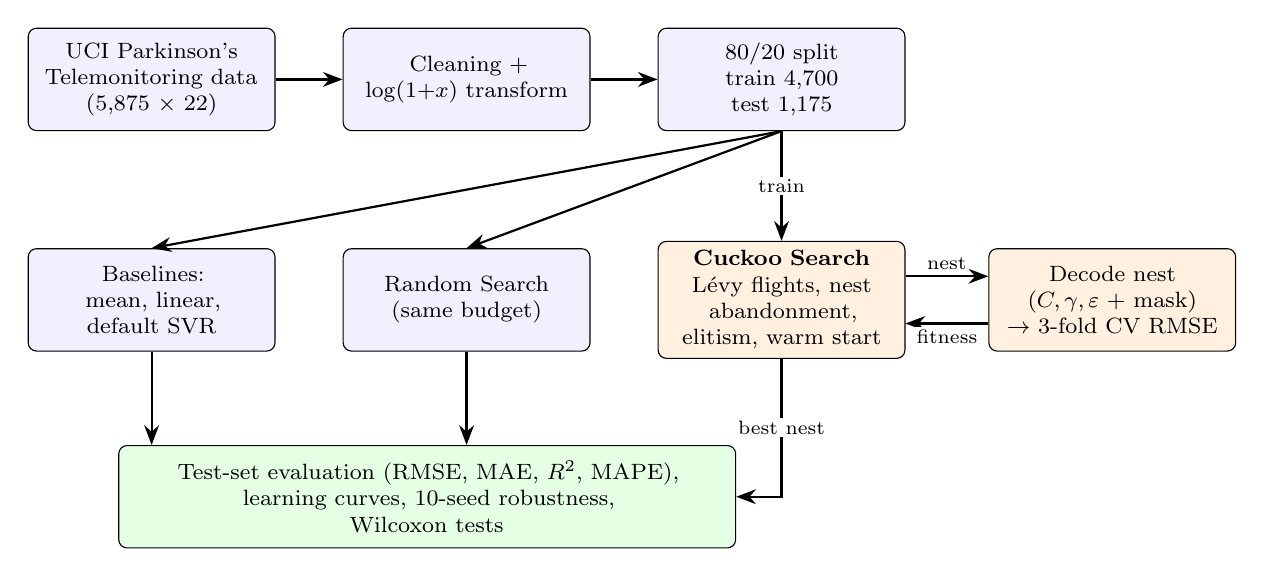
\begin{tikzpicture}[
  box/.style={draw, rounded corners=3pt, align=center, minimum height=1.3cm, text width=2.9cm, font=\footnotesize, fill=blue!6},
  opt/.style={box, fill=orange!12},
  res/.style={box, fill=green!10},
  arr/.style={-{Stealth[length=2.5mm]}, thick},
  lab/.style={font=\scriptsize, fill=white, inner sep=1pt}]
  \node[box] (data) at (0,0) {UCI Parkinson's\\Telemonitoring data\\(5,875 $\times$ 22)};
  \node[box] (prep) at (4,0) {Cleaning +\\$\log(1{+}x)$ transform};
  \node[box] (split) at (8,0) {80/20 split\\train 4,700\\test 1,175};
  \node[box] (base) at (0,-2.8) {Baselines:\\mean, linear,\\default SVR};
  \node[box] (rs) at (4,-2.8) {Random Search\\(same budget)};
  \node[opt] (cs) at (8,-2.8) {\textbf{Cuckoo Search}\\Lévy flights, nest abandonment,\\elitism, warm start};
  \node[opt] (fit) at (12.2,-2.8) {Decode nest\\($C,\gamma,\varepsilon$ + mask)\\$\rightarrow$ 3-fold CV RMSE};
  \node[res, text width=7.6cm] (eval) at (3.5,-5.3) {Test-set evaluation (RMSE, MAE, $R^2$, MAPE),\\learning curves, 10-seed robustness,\\Wilcoxon tests};
  \draw[arr] (data) -- (prep);
  \draw[arr] (prep) -- (split);
  \draw[arr] (split.south) -- node[lab]{train} (cs.north);
  \draw[arr] (split.south) -- (rs.north);
  \draw[arr] (split.south) -- (base.north);
  \draw[arr] ([yshift=3mm]cs.east) -- node[lab, above=1pt]{nest} ([yshift=3mm]fit.west);
  \draw[arr] ([yshift=-3mm]fit.west) -- node[lab, below=1pt]{fitness} ([yshift=-3mm]cs.east);
  \draw[arr] (base.south) -- (base.south |- eval.north);
  \draw[arr] (rs.south) -- (rs.south |- eval.north);
  \draw[arr] (cs.south) |- node[lab, pos=0.25]{best nest} (eval.east);
\end{tikzpicture}
\caption{System architecture of the Cuckoo-optimised SVR pipeline}
\label{fig:arch}
\end{figure}

The system has five modules, each a separate Python file (Table~\ref{tab:code}): data preparation, model definition, search-space encoding and fitness, the optimisers (Cuckoo Search and Random Search), and evaluation and plotting.

\subsection{Dataset}
The Oxford Parkinson's Disease Telemonitoring dataset \cite{tsanas2010} was created by Tsanas and Little (University of Oxford) with ten US medical centres and Intel Corporation, and is available from the UCI Machine Learning Repository. Forty-two people with early-stage PD (28 men, 14 women, aged 36--85) used an at-home device for six months; it recorded sustained phonations of the vowel ``ah'' automatically, about weekly. There are 5,875 recordings in total (101--168 per patient). Clinicians assessed UPDRS at the start, after three months and after six months, and the scores were linearly interpolated to the recording dates.

\begin{table}[H]
\centering
\caption{Dataset attributes}
\label{tab:attrs}
\small
\renewcommand{\arraystretch}{1.15}
\begin{tabularx}{\textwidth}{@{}>{\raggedright}p{5.6cm}>{\raggedright\arraybackslash}Xl@{}}
\toprule
\textbf{Attribute(s)} & \textbf{Description} & \textbf{Role} \\ \midrule
subject\#, test\_time & Patient ID; days since recruitment & Not used \\
age, sex & Demographics (sex: 0 = male, 1 = female) & Feature \\
Jitter(\%), Jitter(Abs), Jitter:RAP, Jitter:PPQ5, Jitter:DDP & Cycle-to-cycle variation of the fundamental frequency & Feature (5) \\
Shimmer, Shimmer(dB), Shimmer:APQ3, APQ5, APQ11, DDA & Cycle-to-cycle variation of amplitude & Feature (6) \\
NHR, HNR & Noise-to-harmonics and harmonics-to-noise ratios & Feature (2) \\
RPDE & Recurrence period density entropy (non-linear complexity) & Feature \\
DFA & Detrended fluctuation analysis (signal fractal scaling) & Feature \\
PPE & Pitch period entropy (non-linear measure of pitch variation) & Feature \\
motor\_UPDRS & Clinician's motor UPDRS score & \textbf{Target} \\
total\_UPDRS & Clinician's total UPDRS score & Not used \\ \bottomrule
\end{tabularx}
\end{table}

The target, motor UPDRS, has mean 21.30, standard deviation 8.13 and range 5.04--39.51 (Figure~\ref{fig:target}). Individually, the features correlate only weakly with the target (Figure~\ref{fig:corr}): the strongest is age ($r = 0.28$), followed by PPE ($0.16$) and HNR ($-0.16$). Within the jitter group and within the shimmer group, features are almost perfectly correlated with each other. Weak individual correlations combined with heavy redundancy indicate that a non-linear model and feature selection are both needed.

\begin{figure}[H]
\centering
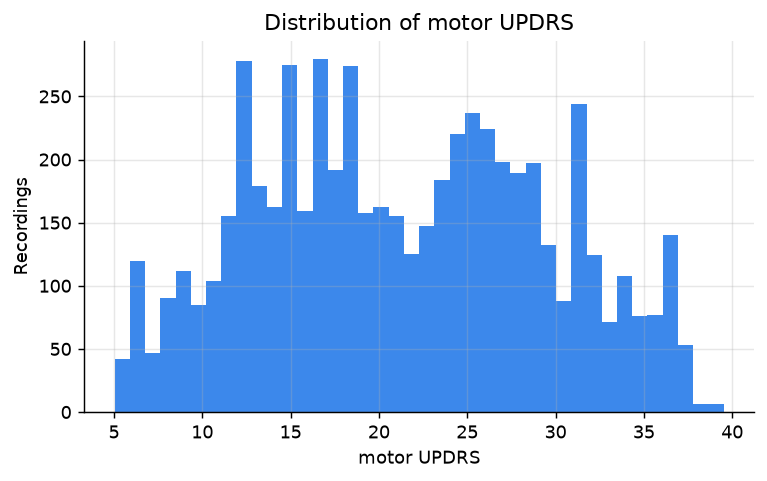
\includegraphics[width=0.62\textwidth]{figures/target_distribution.png}
\caption{Distribution of the target variable (motor UPDRS) over all 5,875 recordings}
\label{fig:target}
\end{figure}

\begin{figure}[H]
\centering
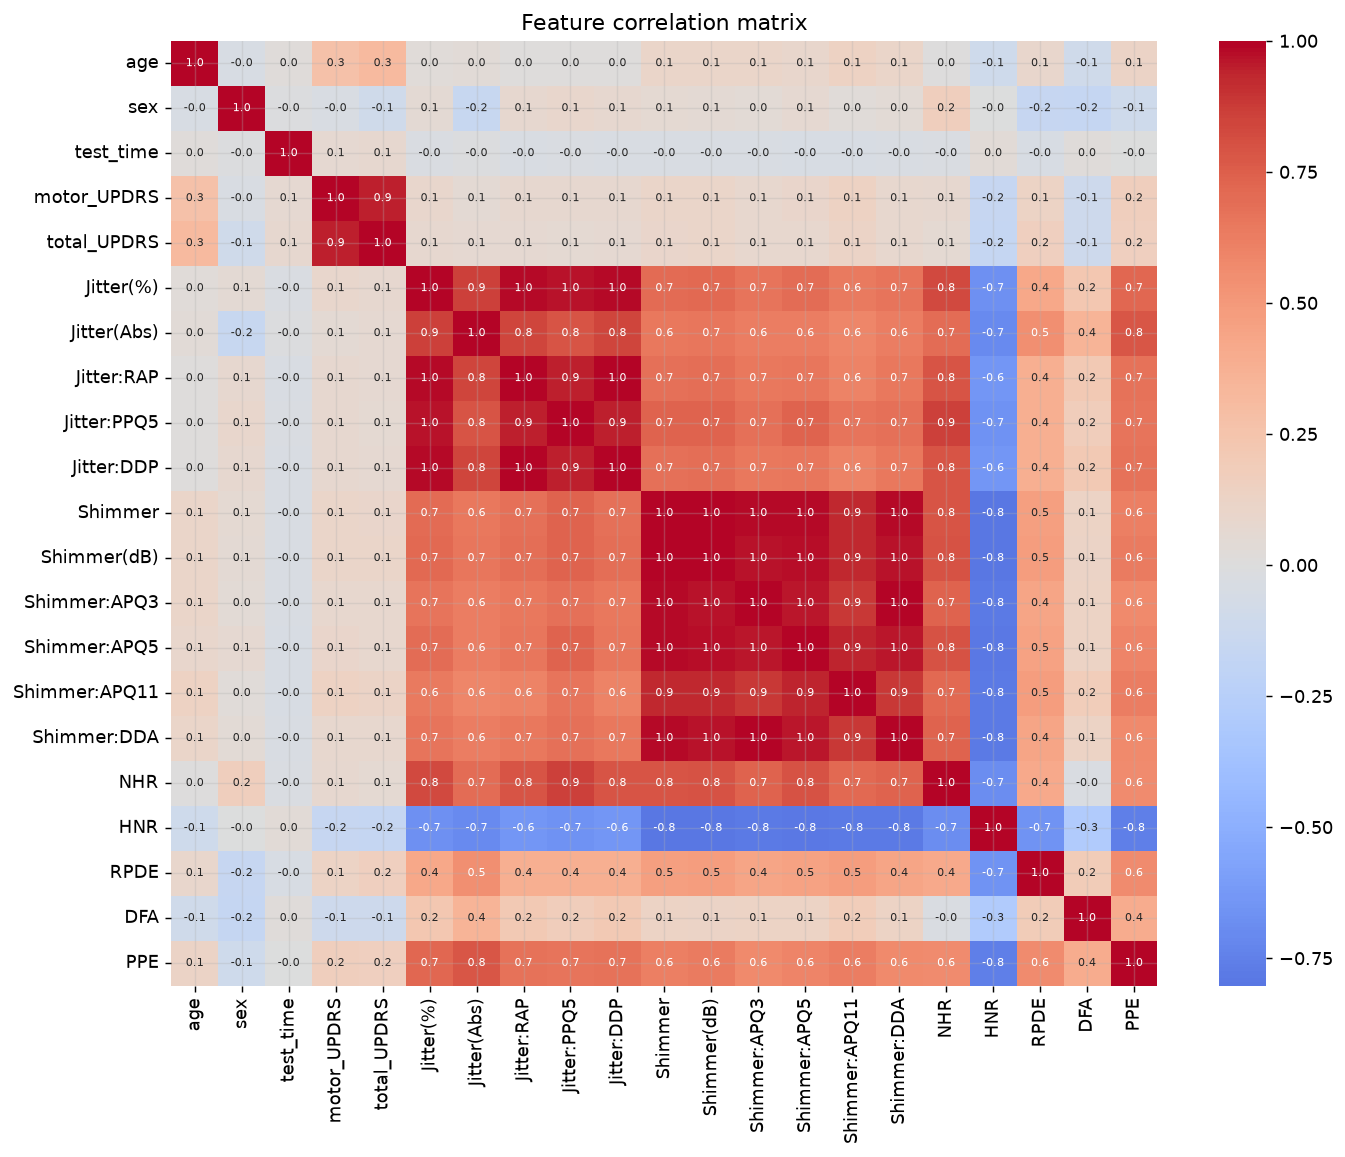
\includegraphics[width=0.7\textwidth]{figures/correlation_heatmap.png}
\caption{Pearson correlation matrix of the features and the target. The jitter and shimmer blocks are highly inter-correlated.}
\label{fig:corr}
\end{figure}

\subsection{Data Preprocessing}
\begin{enumerate}
  \item \textbf{Cleaning.} We checked for missing values and duplicate rows; there are none, so all 5,875 rows are kept.
  \item \textbf{Feature/target separation.} The patient ID, test time and total UPDRS are dropped from the inputs, leaving 18 features; motor UPDRS is the target.
  \item \textbf{Transformation.} The 12 jitter, shimmer and NHR measures are strongly right-skewed and received a $\log(1+x)$ transform. The transform is stateless (it learns nothing from the data), so it cannot leak test information.
  \item \textbf{Splitting.} A random 80/20 split (seed 42) gives 4,700 training and 1,175 test recordings.
  \item \textbf{Scaling.} Features are standardised to zero mean and unit variance, and the target is standardised too, so that $\varepsilon$ is measured in standard deviations. Both scalers sit \emph{inside} the model pipeline, so they are fitted only on the training folds of each cross-validation split.
\end{enumerate}

\begin{table}[H]
\centering
\caption{Preprocessing summary}
\label{tab:prep}
\small
\begin{tabular}{@{}lr@{}}
\toprule
\textbf{Step} & \textbf{Result} \\ \midrule
Raw recordings / patients & 5,875 / 42 \\
Missing values / duplicate rows & 0 / 0 \\
Input features & 18 (age, sex, 16 voice measures) \\
Log-transformed features & 12 (jitter, shimmer, NHR) \\
Training / test recordings & 4,700 / 1,175 \\
Scaling & Standardisation inside the pipeline (features and target) \\ \bottomrule
\end{tabular}
\end{table}

\subsection{Models}
\paragraph{Predictive model.} An $\varepsilon$-SVR with RBF kernel (scikit-learn \cite{pedregosa2011}) inside a pipeline: \texttt{StandardScaler} $\rightarrow$ \texttt{SVR}, wrapped in a \texttt{TransformedTargetRegressor} that standardises the target. SVR was chosen because the problem is small (4,700 samples), non-linear and noisy; SVR's $\varepsilon$-insensitive loss is robust to the label noise introduced by interpolating UPDRS between visits; and its quality depends strongly on hyperparameters, which is exactly what the optimiser is for. It trains in about a second, so hundreds of cross-validated evaluations are affordable on a laptop CPU.

\paragraph{Baselines without optimisation.}
\begin{itemize}
  \item \textbf{Mean predictor:} always predicts the training mean (lower bound on usefulness; $R^2 \approx 0$).
  \item \textbf{Linear regression:} ordinary least squares on all 18 features.
  \item \textbf{Default SVR:} scikit-learn defaults, $C = 1$, $\gamma = $ \texttt{'scale'} ($=1/18$ on standardised data), $\varepsilon = 0.1$, all 18 features. This is the model that Cuckoo Search optimises.
\end{itemize}

\subsection{Solution Encoding}
Each nest is a vector $\mathbf{x} \in [0,1]^{21}$ (Table~\ref{tab:encoding}). The first three components are decoded on a $\log_{10}$ scale,
\begin{equation}
  \theta_k = 10^{\,\log_{10} \ell_k \,+\, x_k \log_{10}(h_k / \ell_k)}, \qquad k = 1,2,3,
\end{equation}
and the remaining 18 by the threshold transfer of Section~3.4. If no feature is selected, the feature with the largest value is kept, so every nest is a valid model.

\begin{table}[H]
\centering
\caption{Nest encoding and hyperparameter search space}
\label{tab:encoding}
\small
\renewcommand{\arraystretch}{1.15}
\begin{tabular}{@{}clccc@{}}
\toprule
\textbf{Dimension(s)} & \textbf{Meaning} & \textbf{Lower} & \textbf{Upper} & \textbf{Decoding} \\ \midrule
1 & $C$ (regularisation) & $10^{-1}$ & $10^{3}$ & $\log_{10}$ scale \\
2 & $\gamma$ (RBF width) & $10^{-4}$ & $10^{1}$ & $\log_{10}$ scale \\
3 & $\varepsilon$ (tube width, standardised units) & $10^{-3}$ & $10^{0}$ & $\log_{10}$ scale \\
4--21 & One bit per feature & 0 & 1 & selected if $x > 0.5$ \\ \bottomrule
\end{tabular}
\end{table}

\subsection{Fitness Function}
\begin{equation}
  f(\mathbf{x}) = \frac{1}{3} \sum_{k=1}^{3} \RMSE_k\big(\mathrm{SVR}_{\boldsymbol{\theta}(\mathbf{x})} \text{ trained on folds} \neq k \text{, using features } \mathbf{m}(\mathbf{x})\big),
\end{equation}
the mean RMSE over a fixed, shuffled 3-fold split of the \emph{training} set (lower is better). The same folds are used for every evaluation and for both optimisers, so fitness values are directly comparable. Every evaluation is logged (hyperparameters, selected features, fitness, best-so-far) for the convergence plots.

\subsection{Cuckoo Search Implementation}
Algorithm~\ref{alg:cs} gives the procedure implemented in \texttt{src/cuckoo.py} (listed in Appendix~\ref{app:code}).

\begin{algorithm}[H]
\caption{Cuckoo Search for joint SVR tuning and feature selection}
\label{alg:cs}
\begin{algorithmic}[1]
\Require fitness $f$, dimension $D = 21$, nests $N$, generations $G$, $p_a$, $\alpha$, $\beta$, warm-start position $\mathbf{x}_{\text{def}}$
\State Initialise nests $\mathbf{x}_1,\dots,\mathbf{x}_N \sim U[0,1]^D$; set $\mathbf{x}_1 \gets \mathbf{x}_{\text{def}}$ \Comment{warm start}
\State Evaluate $f(\mathbf{x}_i)$ for all nests (in parallel)
\For{$g = 1$ \textbf{to} $G$}
  \State $\mathbf{x}_{\text{best}} \gets \arg\min_i f(\mathbf{x}_i)$ \Comment{elitism}
  \For{$i = 1$ \textbf{to} $N$} \Comment{Operator 1: Lévy flights}
    \State $\mathbf{L} \gets$ Mantegna$(\beta)$; \ $\mathbf{z} \sim \mathcal{N}(\mathbf{0},\mathbf{I})$
    \State $\mathbf{x}_i' \gets \mathrm{clip}(\mathbf{x}_i + \alpha\, \mathbf{L} \odot (\mathbf{x}_i - \mathbf{x}_{\text{best}}) \odot \mathbf{z})$
  \EndFor
  \State Evaluate all eggs $f(\mathbf{x}_i')$ in parallel
  \For{$i = 1$ \textbf{to} $N$} \Comment{Operator 2: greedy replacement}
    \If{$f(\mathbf{x}_i') < f(\mathbf{x}_i)$} \ $\mathbf{x}_i \gets \mathbf{x}_i'$ \EndIf
  \EndFor
  \State $H_{ij} \gets \mathbb{1}[u_{ij} < p_a]$; \ permutations $p_1, p_2$; \ $r_i \sim U(0,1)$ \Comment{Operator 3: abandonment}
  \State $\mathbf{x}_i'' \gets \mathrm{clip}(\mathbf{x}_i + r_i (\mathbf{x}_{p_1(i)} - \mathbf{x}_{p_2(i)}) \odot \mathbf{H}_i)$ for every nest with a discovered component
  \State Evaluate rebuilt nests in parallel; keep $\mathbf{x}_i''$ if $f(\mathbf{x}_i'') < f(\mathbf{x}_i)$
  \State Record best and mean fitness of generation $g$
\EndFor
\State \Return $\arg\min_i f(\mathbf{x}_i)$
\end{algorithmic}
\end{algorithm}

\paragraph{Evaluation budget.} A generation costs $N$ egg evaluations plus one per abandoned nest. With $D = 21$ and $p_a = 0.25$, a nest escapes discovery with probability $0.75^{21} \approx 0.24\%$, so almost every nest is rebuilt each generation. With $N = 20$ and $G = 20$ this gives $20 + 20 \times (20 + {\approx}20) \approx 820$ evaluations per run (819 in the main run).

\paragraph{Parallel evaluation.} Each egg depends only on its own nest and the best nest, so all eggs in a generation, and all nests rebuilt by abandonment, are scored as one batch. Every (candidate, fold) SVR fit is dispatched to the 10 CPU cores with \texttt{joblib}. Results are identical to sequential evaluation; we verified that the main run reproduces the same fitness history.

\subsection{Random Search (Non-Bio-Inspired Reference)}
Random Search samples positions uniformly from $[0,1]^{21}$ and decodes them in exactly the same way, so it searches the same space with the same fitness function. For every Cuckoo Search run it receives \emph{exactly} the same number of evaluations. If Cuckoo Search beats it, the gain comes from the bio-inspired operators and not merely from evaluating many configurations.

\subsection{Technology Stack and Code Organisation}
\begin{table}[H]
\centering
\caption{Software and hardware}
\label{tab:stack}
\small
\begin{tabular}{@{}ll@{}}
\toprule
\textbf{Component} & \textbf{Version / detail} \\ \midrule
Python & 3.13.5 \\
NumPy / pandas / SciPy & 2.5.4 / 3.1.0 / 1.18.1 \\
scikit-learn & 1.9.1 (SVR, pipelines, metrics, learning curves) \\
Matplotlib / seaborn & 3.11.2 / 0.13.2 \\
Jupyter (nbconvert) & Executed notebook as record of the run \\
Hardware & Apple M4 (10 CPU cores), 16 GB RAM, no GPU \\ \bottomrule
\end{tabular}
\end{table}

\begin{table}[H]
\centering
\caption{Code organisation}
\label{tab:code}
\small
\renewcommand{\arraystretch}{1.15}
\begin{tabularx}{\textwidth}{@{}l>{\raggedright\arraybackslash}X@{}}
\toprule
\textbf{File} & \textbf{Responsibility} \\ \midrule
\texttt{src/data.py} & Loading, cleaning, log transform, train/test split \\
\texttt{src/model.py} & SVR pipeline (feature + target scaling) and untuned baselines \\
\texttt{src/search\_space.py} & Nest encoding/decoding, CV fitness function with parallel batch evaluation and logging \\
\texttt{src/cuckoo.py} & Cuckoo Search from scratch (Lévy flights, replacement, abandonment, elitism, warm start) \\
\texttt{src/random\_search.py} & Random Search reference optimiser \\
\texttt{src/benchmarks.py} & Sphere, Rastrigin, Rosenbrock, Ackley test functions \\
\texttt{src/metrics.py} & RMSE, MAE, $R^2$, MAPE and before/after comparison tables \\
\texttt{src/plots.py} & All figures \\
\texttt{Parkinsons\_Cuckoo\_SVR.ipynb} & Executed notebook: the complete record of the experiment \\ \bottomrule
\end{tabularx}
\end{table}

\paragraph{Reproducibility.} All randomness (data split, CV folds, optimisers) is seeded; library versions are pinned in \texttt{requirements.txt}; the executed notebook records the run date, machine, library versions and every log line; and all metrics, search logs and figures are saved to \texttt{outputs/}.

% ================================================================= 6 EXPERIMENTAL SETUP
\section{Experimental Setup}\label{sec:setup}

\subsection{Experimental Configuration}
\begin{table}[H]
\centering
\caption{Cuckoo Search and experiment configuration}
\label{tab:config}
\small
\begin{tabular}{@{}lll@{}}
\toprule
\textbf{Parameter} & \textbf{Value} & \textbf{Reason} \\ \midrule
Nests $N$ & 20 & Population size \\
Generations $G$ & 20 & $\approx$820 evaluations per run \\
Discovery probability $p_a$ & 0.25 & Recommended by Yang \& Deb \\
Lévy exponent $\beta$ & 1.5 & Recommended by Yang \& Deb \\
Step scale $\alpha$ & 1.0 & Best of $\{1, 0.1, 0.01\}$ on benchmarks \\
Warm-start nests & 1 (default SVR) & Search starts from the baseline \\
Fitness & 3-fold CV RMSE & Training set only \\
Split seed / main-run seed & 42 / 42 & Reproducibility \\
Robustness seeds & 1--10 & Independent runs \\
Random Search budget & Same as each Cuckoo run & Fair comparison \\ \bottomrule
\end{tabular}
\end{table}

\paragraph{Choice of budget.} An earlier run with only 170 evaluations (10 nests $\times$ 8 generations) left Cuckoo Search and Random Search tied. To see how much budget a guided search needs in 21 dimensions, we ran a budget study on three seeds with about 1,000 evaluations, recording both methods' best-so-far fitness after every evaluation (Table~\ref{tab:budget}). Cuckoo Search was ahead on all three seeds from about 500 evaluations onwards, and the gap kept widening, so the budget was raised to about 820 evaluations \emph{for both methods}.

\begin{table}[H]
\centering
\caption{Budget study: best CV RMSE after a given number of evaluations (CS / RS)}
\label{tab:budget}
\small
\begin{tabular}{@{}ccccc@{}}
\toprule
\textbf{Seed} & \textbf{@170} & \textbf{@500} & \textbf{@750} & \textbf{@$\approx$1020} \\ \midrule
1  & 5.190 / \textbf{4.883} & \textbf{4.546} / 4.727 & \textbf{4.469} / 4.727 & \textbf{4.382} / 4.727 \\
2  & \textbf{4.955} / 5.028 & \textbf{4.594} / 4.928 & \textbf{4.406} / 4.928 & \textbf{4.384} / 4.896 \\
10 & \textbf{4.888} / 5.022 & \textbf{4.745} / 5.022 & \textbf{4.541} / 4.947 & \textbf{4.405} / 4.731 \\ \bottomrule
\end{tabular}
\end{table}

\subsection{Baseline Models}
The three untuned baselines of Section~5.4 are trained on the full training set with all features and evaluated once on the test set. Random Search SVR is the tuned, non-bio-inspired baseline.

\subsection{Test Functions for Validating the Optimiser}\label{sec:testfun}
Before trusting Cuckoo Search on the SVR, we validated its operators on four standard benchmark functions in $D = 10$ dimensions \cite{jamil2013}, each with global minimum $f = 0$:
\begin{align}
  \text{Sphere:} \quad & f(\mathbf{x}) = \textstyle\sum_{i=1}^{D} x_i^2, & x_i \in [-100, 100] \\
  \text{Rastrigin:} \quad & f(\mathbf{x}) = 10D + \textstyle\sum_{i=1}^{D} \big[x_i^2 - 10\cos(2\pi x_i)\big], & x_i \in [-5.12, 5.12] \\
  \text{Rosenbrock:} \quad & f(\mathbf{x}) = \textstyle\sum_{i=1}^{D-1} \big[100(x_{i+1} - x_i^2)^2 + (1 - x_i)^2\big], & x_i \in [-5, 10] \\
  \text{Ackley:} \quad & f(\mathbf{x}) = -20 e^{-0.2\sqrt{\frac{1}{D}\sum x_i^2}} - e^{\frac{1}{D}\sum \cos(2\pi x_i)} + 20 + e, & x_i \in [-32.768, 32.768]
\end{align}
Sphere tests basic convergence; Rastrigin has a huge number of local minima; Rosenbrock has a narrow curved valley; Ackley is nearly flat far from the optimum. Each method was run with 10 seeds and exactly 9,000 evaluations (Cuckoo Search with 25 nests, 200 generations).

\subsection{Cross-Validation Strategy}
\begin{itemize}
  \item \textbf{Fitness during the search:} 3-fold shuffled K-fold on the 4,700 training recordings (fixed folds).
  \item \textbf{Learning curves:} 5-fold shuffled K-fold on the training set with 8 training sizes from 10\% to 100\%.
  \item \textbf{Final evaluation:} the selected model is refitted on all 4,700 training recordings and scored once on the 1,175 test recordings.
\end{itemize}

\subsection{Robustness and Statistical Testing}
Metaheuristics are stochastic, so one good run could be luck. Both optimisers are repeated with 10 different seeds (Cuckoo seeds 1--10, Random Search seeds 1001--1010), each with the same budget, and every resulting model is scored on the test set. We report mean, standard deviation, best and worst test RMSE and the number of wins. One-sided Wilcoxon signed-rank tests check whether Cuckoo Search has lower RMSE than (a) the default SVR and (b) Random Search.

% ================================================================= 7 RESULTS
\section{Results and Discussion}\label{sec:results}

\subsection{Validation of the Cuckoo Search Operators}\label{sec:bench}
Table~\ref{tab:bench} and Figure~\ref{fig:bench} compare Cuckoo Search with Random Search and with an ablation in which a new egg replaces a \emph{randomly chosen} nest (our first implementation).

\begin{table}[H]
\centering
\caption{Benchmark functions ($D=10$, 9,000 evaluations, mean $\pm$ std of best $f$ over 10 seeds; optimum $=0$)}
\label{tab:bench}
\small
\begin{tabular}{@{}lccc@{}}
\toprule
\textbf{Function} & \textbf{Cuckoo Search} & \textbf{CS, random-nest replacement} & \textbf{Random Search} \\ \midrule
Sphere     & $\mathbf{0.019 \pm 0.010}$ & $715 \pm 1200$ & $5413 \pm 756$ \\
Rastrigin  & $\mathbf{16.1 \pm 2.8}$ & $50.4 \pm 14.0$ & $72.4 \pm 6.0$ \\
Rosenbrock & $\mathbf{11.1 \pm 3.6}$ & $712 \pm 733$ & $15169 \pm 4405$ \\
Ackley     & $\mathbf{0.28 \pm 0.13}$ & $11.9 \pm 4.6$ & $17.3 \pm 0.5$ \\ \bottomrule
\end{tabular}
\end{table}

\begin{figure}[H]
\centering
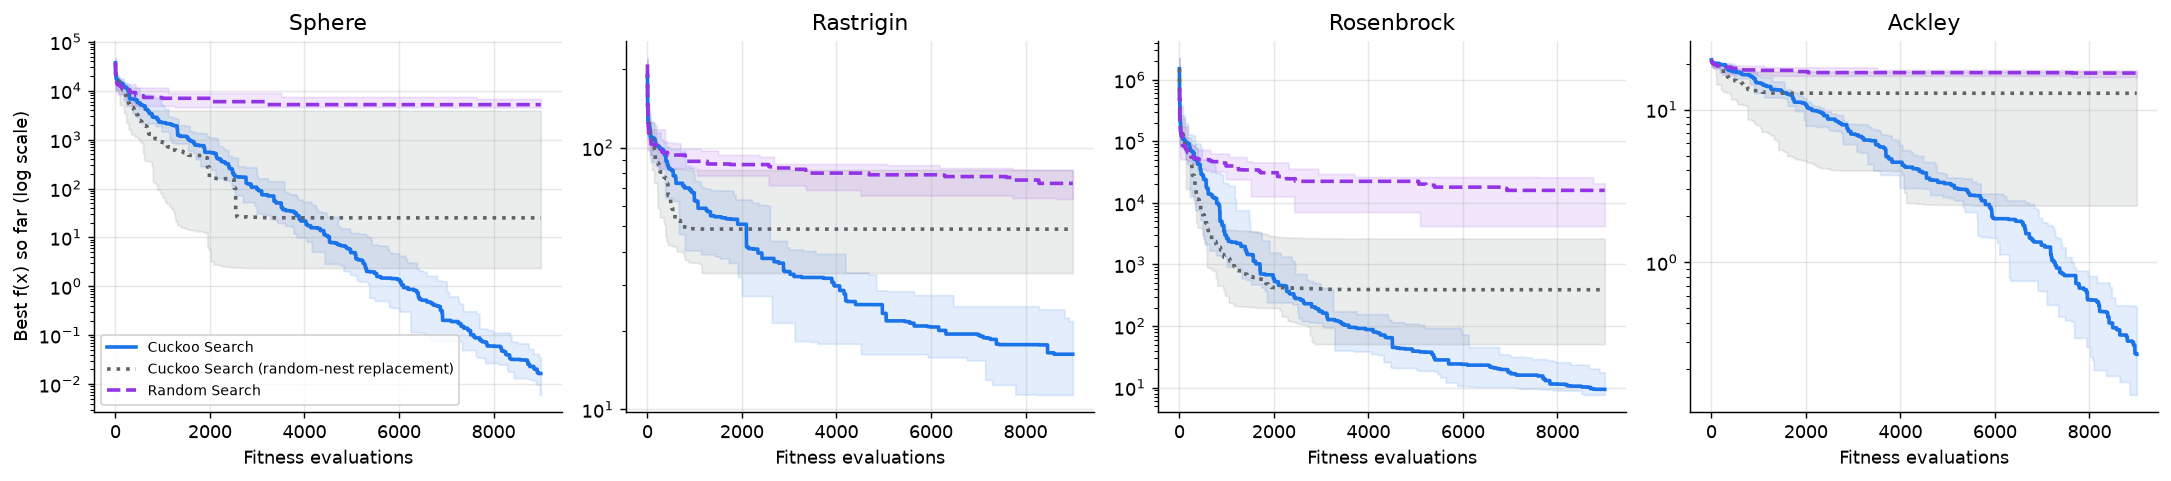
\includegraphics[width=0.85\textwidth]{figures/benchmark_convergence.png}
\caption{Convergence on the benchmark functions (median over 10 seeds; shading spans best to worst run; log scale)}
\label{fig:bench}
\end{figure}

\noindent Observations:
\begin{itemize}
  \item Cuckoo Search beats Random Search on every function, by a factor of about $2.8\times 10^{5}$ on Sphere, $1.4\times 10^{3}$ on Rosenbrock and $60\times$ on Ackley. Its curves keep falling until the budget runs out, showing that the Lévy flights and abandonment keep both exploring and refining.
  \item On Rastrigin, the hardest, highly multi-modal function, Cuckoo Search still lowers the error by $4.5\times$ but does not reach the global optimum within 9,000 evaluations.
  \item The random-nest-replacement variant improves quickly at first and then \emph{flattens}: a good egg is copied into many nests, the population collapses onto one point, and $(\mathbf{x}_i - \mathbf{x}_{\text{best}})$ and $(\mathbf{x}_{p_1} - \mathbf{x}_{p_2})$ shrink to zero, so no operator can move any more. On Sphere it stays about 37,000 times worse. Greedy replacement of the nest's own position fixes this; it is the version used for all SVR results.
\end{itemize}

\subsection{Baseline Results (Without Optimisation)}
\begin{table}[H]
\centering
\caption{Baseline models without optimisation (test set, 1,175 recordings)}
\label{tab:baselines}
\small
\begin{tabular}{@{}lcccc@{}}
\toprule
\textbf{Model} & \textbf{RMSE} & \textbf{MAE} & $\mathbf{R^2}$ & \textbf{MAPE (\%)} \\ \midrule
Mean predictor & 7.991 & 6.878 & $-0.001$ & 43.12 \\
Linear regression & 7.467 & 6.327 & 0.126 & 38.37 \\
Default SVR ($C{=}1$, $\gamma{=}$scale, $\varepsilon{=}0.1$, 18 features) & 5.672 & 4.411 & 0.496 & 26.52 \\ \bottomrule
\end{tabular}
\end{table}
Linear regression explains only 12.6\% of the variance, confirming that the voice--severity relationship is strongly non-linear. The default SVR is much better ($R^2 = 0.50$) but still has an average error of 4.4 UPDRS points.

\subsection{Cuckoo Search Convergence on the SVR}
\begin{figure}[H]
\centering
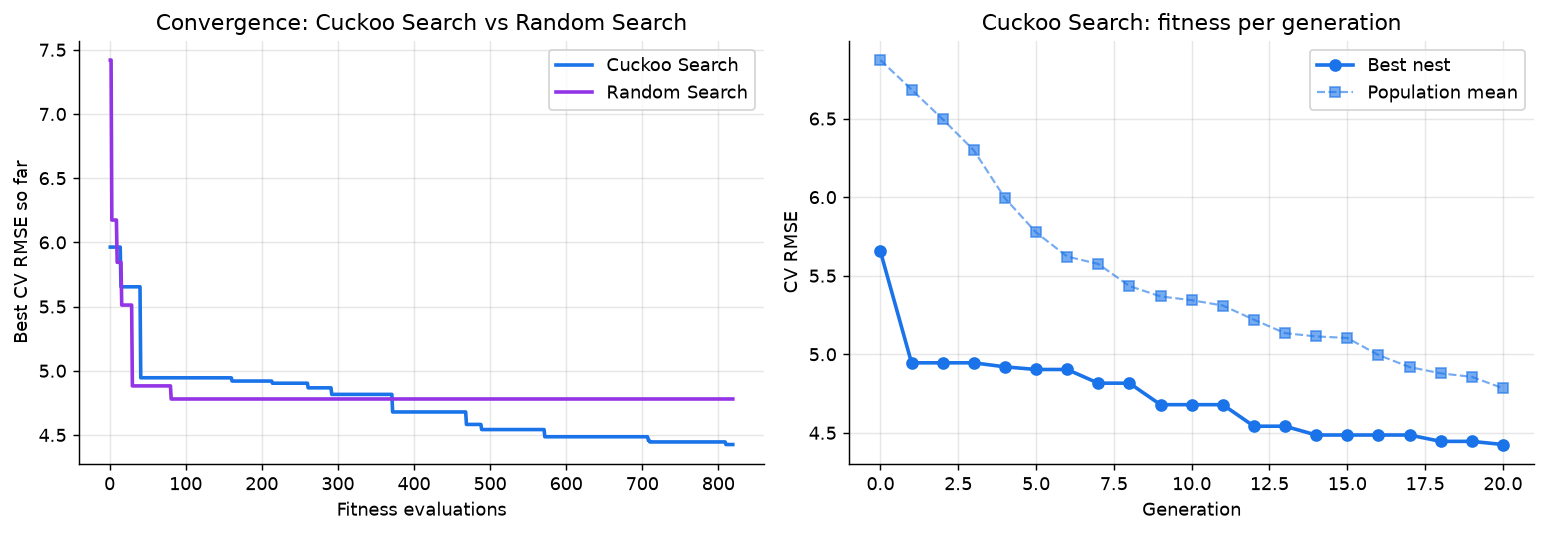
\includegraphics[width=0.85\textwidth]{figures/convergence.png}
\caption{Left: best CV RMSE so far versus fitness evaluations, Cuckoo Search vs Random Search (main run, seed 42). Right: Cuckoo Search best and mean nest fitness per generation.}
\label{fig:conv}
\end{figure}

In the main run (Figure~\ref{fig:conv}) the warm-start nest (default SVR) has a CV RMSE of 5.963. A random initial nest is already better (5.654), and after the first generation the best fitness drops to 4.946. Random Search finds a good configuration early (4.780 after about 80 evaluations) but then stops improving for the remaining 740 evaluations, because uniform sampling rarely lands in the small region of good solutions. Cuckoo Search keeps improving in steps (4.68 at generation 9, 4.54 at 12, 4.49 at 14) and ends at \textbf{4.426}, 7.4\% below Random Search. The population mean (right panel) falls steadily from 6.87 to 4.78, showing that the whole population moves towards better regions rather than one lucky nest.

\subsection{Optimal Configuration}
\begin{table}[H]
\centering
\caption{Configurations of the default, Random Search and Cuckoo Search models}
\label{tab:bestparams}
\small
\begin{tabular}{@{}lccc@{}}
\toprule
\textbf{Parameter} & \textbf{Default SVR} & \textbf{Random Search SVR} & \textbf{Cuckoo-SVR} \\ \midrule
$C$ & 1.0 & 0.692 & 15.68 \\
$\gamma$ & 0.0556 (scale) & 1.866 & 0.825 \\
$\varepsilon$ & 0.1 & 0.0020 & 0.0394 \\
Features used & 18 & 8 & \textbf{9} \\
CV RMSE (training) & 5.963 & 4.780 & \textbf{4.426} \\ \bottomrule
\end{tabular}
\end{table}

The Cuckoo-SVR selected \textit{age, sex, Jitter(\%), Jitter(Abs), Jitter:DDP, Shimmer, NHR, HNR} and \textit{DFA}. Compared with the default, it uses a much larger $C$ (fits the data more closely) and a $15\times$ larger $\gamma$ (a more local kernel). This combination only works because half of the redundant features are removed; with all 18 features, distances between recordings are dominated by the near-duplicate jitter and shimmer measures.

\subsection{Comparison: Baseline vs Optimised Model}
\begin{table}[H]
\centering
\caption{All models on the test set (main run)}
\label{tab:all}
\small
\begin{tabular}{@{}lcccc@{}}
\toprule
\textbf{Model} & \textbf{RMSE} & \textbf{MAE} & $\mathbf{R^2}$ & \textbf{MAPE (\%)} \\ \midrule
Mean predictor & 7.991 & 6.878 & $-0.001$ & 43.12 \\
Linear regression & 7.467 & 6.327 & 0.126 & 38.37 \\
Default SVR & 5.672 & 4.411 & 0.496 & 26.52 \\
Random Search SVR & 4.693 & 3.297 & 0.655 & 19.51 \\
\textbf{Cuckoo-SVR (proposed)} & \textbf{4.347} & \textbf{3.066} & \textbf{0.704} & \textbf{17.97} \\ \bottomrule
\end{tabular}
\end{table}

\begin{table}[H]
\centering
\caption{Improvement of the Cuckoo-SVR over the default SVR and over Random Search SVR}
\label{tab:improve}
\small
\begin{tabular}{@{}lcccc@{}}
\toprule
& \multicolumn{2}{c}{\textbf{vs default SVR}} & \multicolumn{2}{c}{\textbf{vs Random Search SVR}} \\
\cmidrule(lr){2-3}\cmidrule(lr){4-5}
\textbf{Metric} & \textbf{Change} & \textbf{Improvement} & \textbf{Change} & \textbf{Improvement} \\ \midrule
RMSE & $5.672 \rightarrow 4.347$ & 23.4\% & $4.693 \rightarrow 4.347$ & 7.4\% \\
MAE & $4.411 \rightarrow 3.066$ & 30.5\% & $3.297 \rightarrow 3.066$ & 7.0\% \\
$R^2$ & $0.496 \rightarrow 0.704$ & +0.208 (42.0\%) & $0.655 \rightarrow 0.704$ & +0.049 (7.5\%) \\
MAPE & $26.52 \rightarrow 17.97$\% & 32.2\% & $19.51 \rightarrow 17.97$\% & 7.9\% \\
Features & $18 \rightarrow 9$ & 50\% fewer & $8 \rightarrow 9$ & -- \\ \bottomrule
\end{tabular}
\end{table}

\begin{figure}[H]
\centering
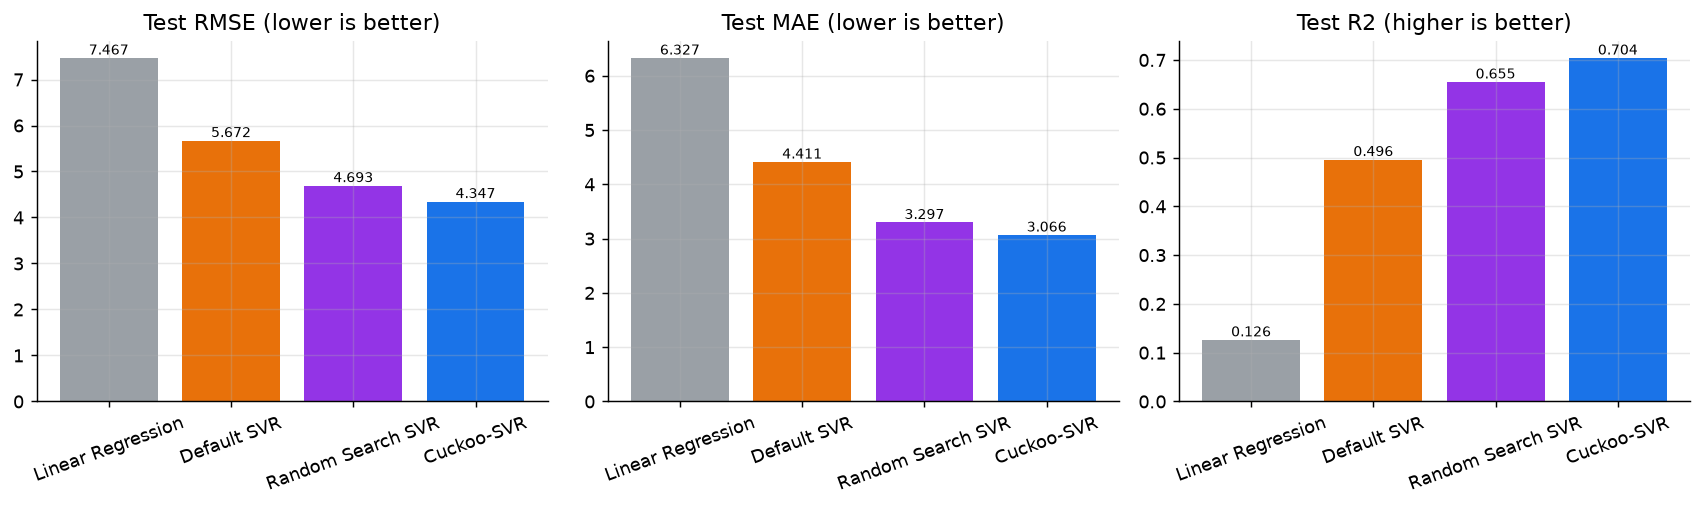
\includegraphics[width=0.8\textwidth]{figures/metric_comparison.png}
\caption{Test RMSE, MAE and $R^2$ of the linear, default SVR, Random Search SVR and Cuckoo-SVR models}
\label{fig:bars}
\end{figure}

Cuckoo Search improves on the default SVR on every metric: the RMSE falls by 1.33 UPDRS points (23.4\%), the MAE by 30.5\%, and the explained variance rises from 50\% to 70\%. It also beats the tuned Random Search model on every metric by about 7\%.

\subsection{Prediction Quality and Error Analysis}
\begin{figure}[H]
\centering
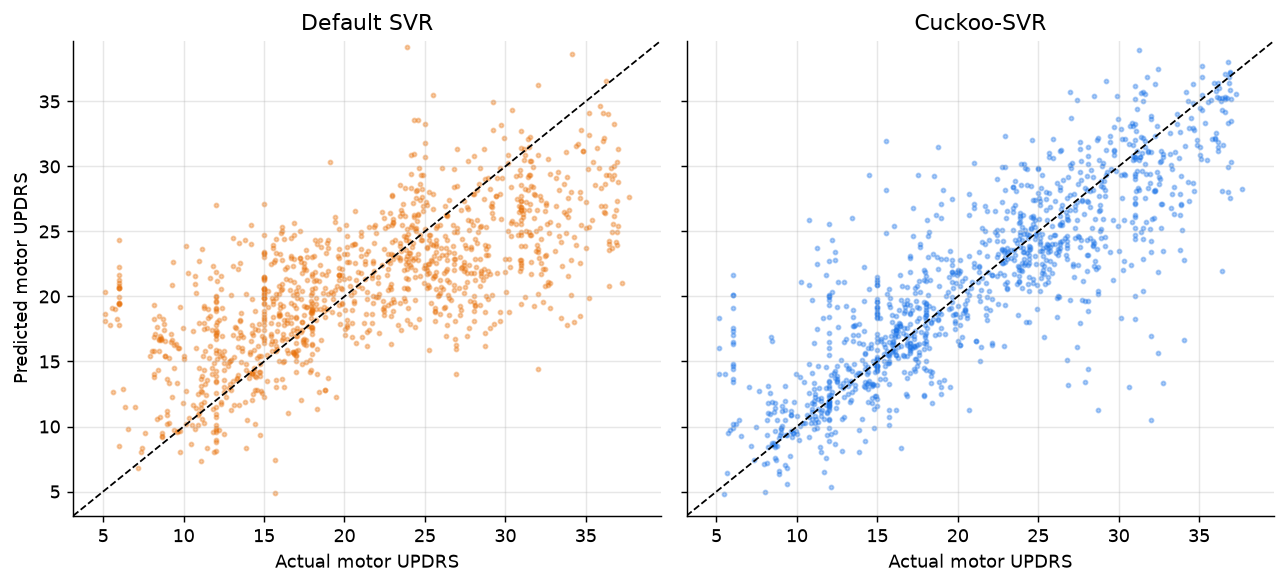
\includegraphics[width=0.8\textwidth]{figures/predicted_vs_actual.png}
\caption{Predicted versus actual motor UPDRS on the test set. The dashed line is a perfect prediction.}
\label{fig:pva}
\end{figure}

The default SVR (Figure~\ref{fig:pva}, left) shows the typical shrinkage of an over-smoothed model: it overestimates mild cases and underestimates severe ones, so its points form a band flatter than the diagonal. The Cuckoo-SVR's points lie much closer to the diagonal across the whole range. Its residuals are centred at zero (mean 0.01 versus 0.23) and are narrower (standard deviation 4.35 versus 5.67), and 80.8\% of its predictions are within 5 UPDRS points of the clinician's score, compared with 63.7\% for the default. The residual distribution has heavier tails (excess kurtosis 2.6): most errors are small, with a few larger misses.

\begin{table}[H]
\centering
\caption{Test error by disease severity}
\label{tab:severity}
\small
\begin{tabular}{@{}lccccc@{}}
\toprule
& & \multicolumn{2}{c}{\textbf{Default SVR}} & \multicolumn{2}{c}{\textbf{Cuckoo-SVR}} \\
\cmidrule(lr){3-4}\cmidrule(lr){5-6}
\textbf{Motor UPDRS range} & \textbf{Recordings} & \textbf{RMSE} & \textbf{MAE} & \textbf{RMSE} & \textbf{MAE} \\ \midrule
Mild ($<15$) & 291 & 6.458 & 4.915 & \textbf{4.708} & \textbf{3.144} \\
Moderate (15--25) & 476 & 3.810 & 3.002 & \textbf{3.431} & \textbf{2.510} \\
Severe ($\ge 25$) & 408 & 6.781 & 5.697 & \textbf{4.986} & \textbf{3.659} \\ \bottomrule
\end{tabular}
\end{table}

Table~\ref{tab:severity} confirms this: the largest gains are at the extremes (MAE drops by 36\% for mild and severe cases), exactly where the default model regressed towards the mean. Mild and severe cases remain harder than moderate ones because there are fewer training examples there.

\subsection{Learning Curves}
\begin{figure}[H]
\centering
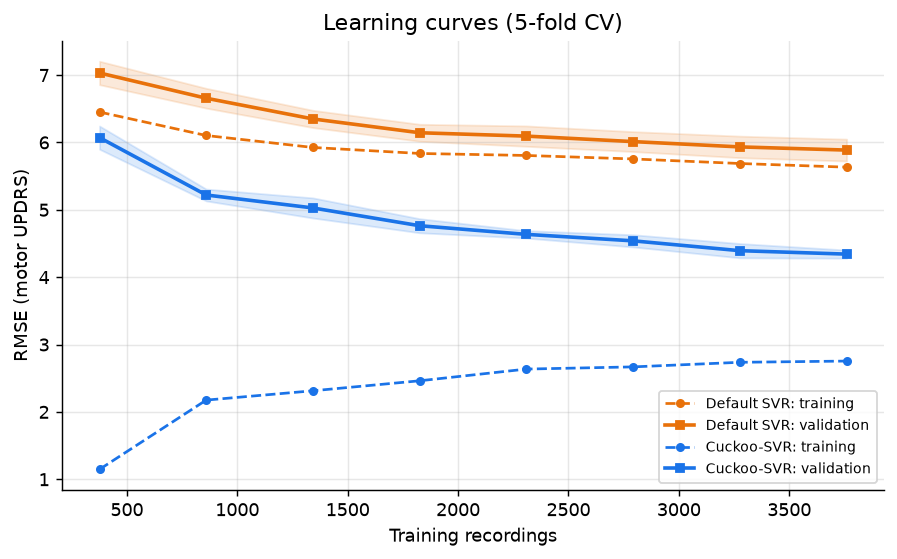
\includegraphics[width=0.75\textwidth]{figures/learning_curves.png}
\caption{Learning curves: training and 5-fold validation RMSE versus training-set size (shaded: $\pm 1$ std over folds)}
\label{fig:lc}
\end{figure}

\begin{table}[H]
\centering
\caption{Learning-curve values (RMSE, mean over 5 folds)}
\label{tab:lc}
\small
\begin{tabular}{@{}rcccc@{}}
\toprule
& \multicolumn{2}{c}{\textbf{Default SVR}} & \multicolumn{2}{c}{\textbf{Cuckoo-SVR}} \\
\cmidrule(lr){2-3}\cmidrule(lr){4-5}
\textbf{Training recordings} & \textbf{Train} & \textbf{Validation} & \textbf{Train} & \textbf{Validation} \\ \midrule
376   & 6.451 & 7.031 & 1.147 & 6.071 \\
1,342 & 5.925 & 6.349 & 2.314 & 5.028 \\
2,309 & 5.807 & 6.094 & 2.636 & 4.635 \\
3,276 & 5.687 & 5.934 & 2.736 & 4.393 \\
3,760 & 5.633 & 5.886 & 2.755 & \textbf{4.342} \\ \bottomrule
\end{tabular}
\end{table}

The learning curves (Figure~\ref{fig:lc}, Table~\ref{tab:lc}) diagnose the two models:
\begin{itemize}
  \item \textbf{Default SVR: underfitting (high bias).} Training and validation errors are close together and both high (5.6--5.9); more data helps only slightly. The model is too smooth to capture the relationship.
  \item \textbf{Cuckoo-SVR: low bias, decreasing variance.} The training error is much lower (2.8), and the validation error falls steadily from 6.07 to 4.34 as data is added and has not levelled off. The gap between the curves shows some variance, which is expected for a flexible RBF model, but the validation error is below the default at every training size.
\end{itemize}
The still-falling validation curve suggests the optimised model would benefit from more recordings.

\subsection{Robustness Across Independent Runs}
\begin{table}[H]
\centering
\caption{Test RMSE of 10 independent runs of each optimiser (same budget per run)}
\label{tab:seeds}
\small
\begin{tabular}{@{}cccccc@{}}
\toprule
\textbf{Seed} & \textbf{Cuckoo Search} & \textbf{Random Search} & \textbf{Better} & \textbf{CS features} & \textbf{CS $R^2$} \\ \midrule
1  & \textbf{4.361} & 4.610 & CS & 11 & 0.702 \\
2  & \textbf{4.302} & 4.727 & CS & 9  & 0.710 \\
3  & \textbf{4.351} & 4.753 & CS & 8  & 0.703 \\
4  & \textbf{4.327} & 4.504 & CS & 9  & 0.707 \\
5  & 4.400 & \textbf{4.370} & RS & 9  & 0.697 \\
6  & \textbf{4.303} & 4.871 & CS & 9  & 0.710 \\
7  & \textbf{4.324} & 4.455 & CS & 9  & 0.707 \\
8  & \textbf{4.419} & 4.604 & CS & 8  & 0.694 \\
9  & \textbf{4.380} & 4.763 & CS & 9  & 0.699 \\
10 & 4.395 & \textbf{4.303} & RS & 11 & 0.697 \\ \bottomrule
\end{tabular}
\end{table}

\begin{table}[H]
\centering
\caption{Robustness summary and statistical tests}
\label{tab:robust}
\small
\begin{tabular}{@{}lcc@{}}
\toprule
& \textbf{Cuckoo Search} & \textbf{Random Search} \\ \midrule
Mean test RMSE & \textbf{4.356} & 4.596 \\
Standard deviation & \textbf{0.042} & 0.186 \\
Best / worst run & 4.302 / \textbf{4.419} & 4.303 / 4.871 \\
Runs beating the default SVR (5.672) & 10/10 & 10/10 \\
Mean improvement over default SVR & \textbf{23.2\%} & 19.0\% \\
Runs beating the other method & \textbf{8/10} & 2/10 \\ \midrule
Wilcoxon (one-sided): CS $<$ default SVR & \multicolumn{2}{c}{$p = 0.00098$} \\
Wilcoxon (one-sided): CS $<$ Random Search & \multicolumn{2}{c}{$p = 0.0049$} \\ \bottomrule
\end{tabular}
\end{table}

\begin{figure}[H]
\centering
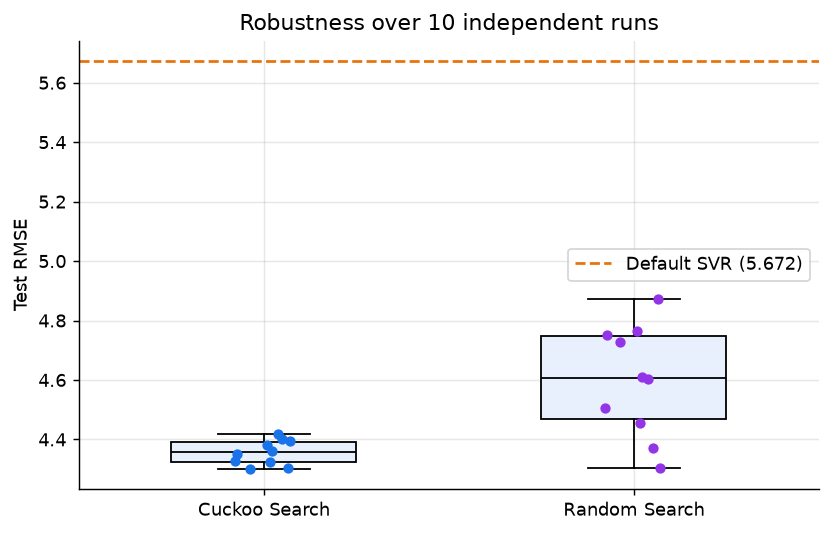
\includegraphics[width=0.66\textwidth]{figures/robustness_boxplot.png}
\caption{Test RMSE over 10 independent runs of each optimiser, against the default SVR (dashed line)}
\label{fig:box}
\end{figure}

The improvement is not a lucky run. Cuckoo Search beats the default SVR in all 10 runs ($p = 0.00098$, the smallest $p$-value possible with 10 pairs) and beats Random Search in 8 of 10 ($p = 0.0049$, significant at the 1\% level). Just as important, it is far more \emph{consistent}: its standard deviation (0.042) is 4.4 times smaller than Random Search's (0.186), and its \emph{worst} run (4.419) is better than Random Search's \emph{average} (4.596). Random Search occasionally samples a very good configuration by chance (seeds 5 and 10) but often does not (seed 6: 4.871). Cuckoo Search finds a good configuration every time.

\subsection{Feature Selection Results}
\begin{figure}[H]
\centering
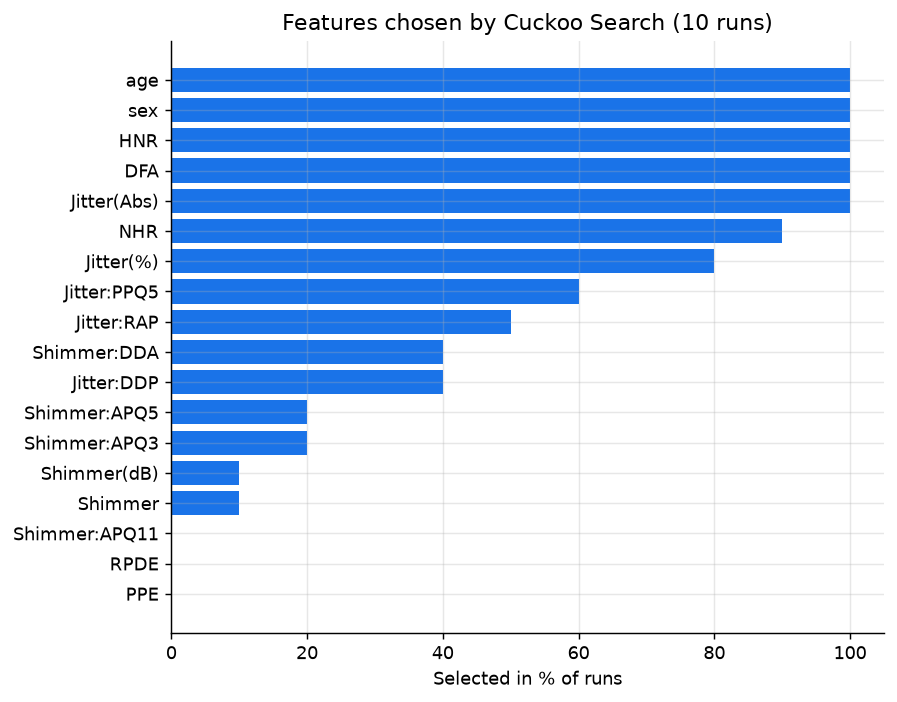
\includegraphics[width=0.66\textwidth]{figures/feature_selection_frequency.png}
\caption{How often each feature was selected across the 10 Cuckoo Search runs}
\label{fig:feat}
\end{figure}

Across the 10 runs Cuckoo Search kept 8--11 features (Figure~\ref{fig:feat}). Age, sex, HNR, DFA and Jitter(Abs) were chosen in \emph{every} run, NHR in 9 runs and Jitter(\%) in 8. Most shimmer variants were dropped, and Shimmer:APQ11, RPDE and PPE were never selected. This makes sense: the jitter and shimmer families are near-duplicates (Figure~\ref{fig:corr}), so one or two representatives carry the information. Interestingly, PPE and RPDE, which have relatively high individual correlations with UPDRS, were dropped, which suggests their information is already captured by the selected combination. The consistency of the selected subset across independent runs is further evidence that the search converges to a genuine optimum rather than random noise.

\subsection{Computational Performance}
On an Apple M4 laptop (10 CPU cores) the benchmark study took 6\,s, the main Cuckoo Search run 12.2\,min (819 evaluations), the main Random Search run 7.1\,min, the learning curves 8\,s and the robustness study (10 seeds $\times$ 2 optimisers) 153.7\,min, for a total notebook run of 173.2\,min. A single evaluation (three SVR fits) takes about 0.5--1 s. Cuckoo Search is slower per evaluation than Random Search because it concentrates on the high-$C$, high-$\gamma$ region where SVR fits take longer, while many random samples have small $C$ and train quickly. The whole optimisation runs on a laptop CPU without a GPU.

\subsection{Development and Validation History}
The final results came from three versions of the experiment; all are saved in the project's \texttt{archive/} folder for transparency.
\begin{table}[H]
\centering
\caption{Versions of the experiment}
\label{tab:history}
\small
\renewcommand{\arraystretch}{1.15}
\begin{tabularx}{\textwidth}{@{}c>{\raggedright}X>{\raggedright\arraybackslash}X@{}}
\toprule
\textbf{Version} & \textbf{Setup} & \textbf{Outcome} \\ \midrule
v1 & Random-nest replacement, 170 evaluations & Beat default SVR (10/10); beat Random Search in 7/10 ($p = 0.12$, not significant) \\
v2 & Greedy replacement (bug fixed), 170 evaluations & Beat default SVR (10/10); tied with Random Search (4/10): budget too small \\
v3 & Greedy replacement, $\approx$820 evaluations & Beat default SVR (10/10) and Random Search (8/10, $p = 0.005$) \\ \bottomrule
\end{tabularx}
\end{table}
The benchmark study (Section~\ref{sec:bench}) exposed the population-collapse problem of v1. v1 looked reasonable at 170 evaluations only because collapsing fast is a decent strategy for a very short search. The v2 tie showed that 8 generations are too few for a guided search to pay off in 21 dimensions; the budget study (Table~\ref{tab:budget}) set the final budget. In every version the optimised model beat the untuned default.

\subsection{Discussion}

\paragraph{Why Cuckoo Search works well here.}
\begin{enumerate}
  \item \textbf{Joint optimisation.} Hyperparameters and features interact: the large $\gamma$ the search found only works with redundant features removed. Optimising them together finds combinations that tuning either alone would miss.
  \item \textbf{Adaptive step sizes.} Because steps scale with $(\mathbf{x}_i - \mathbf{x}_{\text{best}})$, the search takes large steps early and fine steps late, which produces the steady improvements in Figure~\ref{fig:conv}.
  \item \textbf{Diversity through abandonment.} Rebuilding nests from differences between other nests keeps the population spread out, so the search does not stall (in contrast to the ablation in Figure~\ref{fig:bench}).
  \item \textbf{Warm start and greedy selection.} Starting from the default model and never accepting a worse nest guarantees the result is at least as good as the baseline in cross-validation.
\end{enumerate}

\paragraph{Limitations.}
\begin{itemize}
  \item \textbf{Random split across patients.} Each patient contributes about 140 recordings, and the random split places recordings of the same patient in both training and test sets. The results therefore measure accuracy for monitoring \emph{patients already seen by the model}, which is the telemonitoring scenario, not for diagnosing new patients. In a preliminary check with a patient-wise split, all models (including the baselines) failed to generalise to unseen patients ($R^2 < 0$), because 42 patients are too few to learn between-patient differences.
  \item \textbf{Weak log transform.} Many jitter and shimmer values are much smaller than 1, so $\log(1+x) \approx x$ and the skewness was barely reduced (e.g.\ Jitter(\%): 6.45 before, 6.08 after). A plain logarithm would be more effective.
  \item \textbf{Computational cost.} Each fitness evaluation requires three SVR fits; the full robustness study took 2.6 hours on 10 cores.
  \item \textbf{Single objective.} The fitness uses only CV RMSE; the number of features is reduced as a side effect, not explicitly rewarded.
  \item \textbf{Interpolated targets.} UPDRS was measured only three times per patient and interpolated, which adds label noise and caps achievable accuracy.
\end{itemize}

\paragraph{Practical implications.} With an average error of about 3 UPDRS points and 81\% of predictions within 5 points, a Cuckoo-optimised SVR trained on a patient's earlier, clinician-labelled recordings could track that patient's motor symptoms between clinic visits from a short voice recording, flagging significant deterioration for review. It would support, not replace, clinical assessment.

% ================================================================= 8 CONCLUSION
\section{Conclusion}\label{sec:conclusion}

This project applied Cuckoo Search, a nature-inspired metaheuristic based on the brood parasitism of cuckoos, to optimise a Support Vector Regressor that predicts Parkinson's disease motor severity (motor UPDRS) from voice recordings. Cuckoo Search was implemented from scratch with all of its operators---Lévy flights via Mantegna's algorithm, greedy nest replacement, nest abandonment, elitism and a warm start---and used to tune $C$, $\gamma$ and $\varepsilon$ while selecting the input features.

The key findings are:
\begin{enumerate}
  \item \textbf{Validated optimiser.} On four benchmark functions Cuckoo Search outperformed Random Search by up to five orders of magnitude, and an ablation showed that greedy per-nest replacement is essential to avoid population collapse.
  \item \textbf{Large improvement over the baseline.} The optimised SVR reduced test RMSE from 5.672 to 4.347 (23.4\%), MAE by 30.5\% and MAPE by 32.2\%, and increased $R^2$ from 0.496 to 0.704.
  \item \textbf{Simpler model.} It used only 9 of the 18 features; age, sex, HNR, DFA and Jitter(Abs) were selected in every run.
  \item \textbf{Better than Random Search with the same budget.} Over 10 runs Cuckoo Search achieved a mean test RMSE of $4.356 \pm 0.042$ versus $4.596 \pm 0.186$, winning 8/10 runs (Wilcoxon $p = 0.005$).
  \item \textbf{Robust.} It beat the default SVR in all 10 runs ($p = 0.001$), and its worst run was better than Random Search's average.
  \item \textbf{Diagnosed models.} Learning curves showed that the default SVR underfits, while the optimised model has low bias and keeps improving with more data.
\end{enumerate}
Overall, Cuckoo Search proved to be an effective, low-parameter and reproducible method for joint hyperparameter tuning and feature selection, and the optimised model brings voice-based remote monitoring of Parkinson's disease closer to practical use.

% ================================================================= 9 FUTURE WORK
\section{Future Work}\label{sec:future}

\subsection{Methodological Enhancements}
\paragraph{Generalisation to new patients.} Evaluate with patient-wise (grouped) cross-validation on a larger cohort, or personalise the model with a few labelled recordings of each new patient.

\paragraph{Better preprocessing.} Replace $\log(1+x)$ with a plain logarithm or a Yeo--Johnson power transform to reduce the skewness of the jitter, shimmer and NHR measures.

\paragraph{Multi-objective optimisation.} Minimise RMSE and the number of features simultaneously (e.g.\ with a multi-objective Cuckoo Search or NSGA-II) to obtain a Pareto front of accuracy--simplicity trade-offs.

\paragraph{Algorithm improvements.} Adaptive $p_a$ and $\alpha$ that shrink over the generations, an S- or V-shaped transfer function for the feature bits \cite{mirjalili2013}, and hybrids with Differential Evolution or local search to refine the final solution.

\paragraph{Comparison with other optimisers.} Compare against GA, PSO, DE and Bayesian optimisation with the same budget and statistical protocol.

\subsection{Model Extensions}
\paragraph{Other models.} Apply the same framework to gradient-boosted trees or small neural networks, and to predicting total UPDRS.

\paragraph{Richer inputs.} Use the raw recordings with learned audio features (e.g.\ MFCCs or spectrogram CNNs), with Cuckoo Search tuning the feature extractor as well as the regressor.

% ================================================================= REFERENCES
\newpage
\addcontentsline{toc}{section}{References}
\begin{thebibliography}{99}
\footnotesize\sloppy\setlength{\itemsep}{1pt}
\bibitem{yang2009} X.-S. Yang and S. Deb, ``Cuckoo search via Lévy flights,'' in \emph{Proc. World Congress on Nature \& Biologically Inspired Computing (NaBIC)}, IEEE, 2009, pp.\ 210--214.
\bibitem{yang2010eng} X.-S. Yang and S. Deb, ``Engineering optimisation by cuckoo search,'' \emph{Int. J. Mathematical Modelling and Numerical Optimisation}, vol.\ 1, no.\ 4, pp.\ 330--343, 2010.
\bibitem{yang2010book} X.-S. Yang, \emph{Nature-Inspired Metaheuristic Algorithms}, 2nd ed. Luniver Press, 2010.
\bibitem{mantegna1994} R. N. Mantegna, ``Fast, accurate algorithm for numerical simulation of Lévy stable stochastic processes,'' \emph{Physical Review E}, vol.\ 49, no.\ 5, pp.\ 4677--4683, 1994.
\bibitem{tsanas2010} A. Tsanas, M. A. Little, P. E. McSharry and L. O. Ramig, ``Accurate telemonitoring of Parkinson's disease progression by noninvasive speech tests,'' \emph{IEEE Trans. Biomedical Engineering}, vol.\ 57, no.\ 4, pp.\ 884--893, 2010.
\bibitem{little2009} M. A. Little, P. E. McSharry, E. J. Hunter, J. Spielman and L. O. Ramig, ``Suitability of dysphonia measurements for telemonitoring of Parkinson's disease,'' \emph{IEEE Trans. Biomedical Engineering}, vol.\ 56, no.\ 4, pp.\ 1015--1022, 2009.
\bibitem{sakar2013} B. E. Sakar et al., ``Collection and analysis of a Parkinson speech dataset with multiple types of sound recordings,'' \emph{IEEE J. Biomedical and Health Informatics}, vol.\ 17, no.\ 4, pp.\ 828--834, 2013.
\bibitem{eskidere2012} Ö. Eskidere, F. Ertaş and C. Hanilçi, ``A comparison of regression methods for remote tracking of Parkinson's disease progression,'' \emph{Expert Systems with Applications}, vol.\ 39, no.\ 5, pp.\ 5523--5528, 2012.
\bibitem{goetz2008} C. G. Goetz et al., ``Movement Disorder Society-sponsored revision of the Unified Parkinson's Disease Rating Scale (MDS-UPDRS),'' \emph{Movement Disorders}, vol.\ 23, no.\ 15, pp.\ 2129--2170, 2008.
\bibitem{poewe2017} W. Poewe et al., ``Parkinson disease,'' \emph{Nature Reviews Disease Primers}, vol.\ 3, 17013, 2017.
\bibitem{vapnik1995} V. N. Vapnik, \emph{The Nature of Statistical Learning Theory}. Springer, 1995.
\bibitem{smola2004} A. J. Smola and B. Schölkopf, ``A tutorial on support vector regression,'' \emph{Statistics and Computing}, vol.\ 14, no.\ 3, pp.\ 199--222, 2004.
\bibitem{hsu2003} C.-W. Hsu, C.-C. Chang and C.-J. Lin, ``A practical guide to support vector classification,'' Technical report, Dept.\ of Computer Science, National Taiwan University, 2003.
\bibitem{bergstra2012} J. Bergstra and Y. Bengio, ``Random search for hyper-parameter optimization,'' \emph{J. Machine Learning Research}, vol.\ 13, pp.\ 281--305, 2012.
\bibitem{snoek2012} J. Snoek, H. Larochelle and R. P. Adams, ``Practical Bayesian optimization of machine learning algorithms,'' in \emph{Advances in Neural Information Processing Systems 25}, 2012.
\bibitem{huang2006} C.-L. Huang and C.-J. Wang, ``A GA-based feature selection and parameters optimization for support vector machines,'' \emph{Expert Systems with Applications}, vol.\ 31, no.\ 2, pp.\ 231--240, 2006.
\bibitem{lin2008} S.-W. Lin, K.-C. Ying, S.-C. Chen and Z.-J. Lee, ``Particle swarm optimization for parameter determination and feature selection of support vector machines,'' \emph{Expert Systems with Applications}, vol.\ 35, no.\ 4, pp.\ 1817--1824, 2008.
\bibitem{rodrigues2013} D. Rodrigues, L. A. M. Pereira, A. N. Souza, C. C. Ramos and X.-S. Yang, ``Binary cuckoo search: a binary cuckoo search algorithm for feature selection,'' in \emph{Proc. IEEE Int. Symposium on Circuits and Systems (ISCAS)}, 2013, pp.\ 465--468.
\bibitem{mirjalili2013} S. Mirjalili and A. Lewis, ``S-shaped versus V-shaped transfer functions for binary particle swarm optimization,'' \emph{Swarm and Evolutionary Computation}, vol.\ 9, pp.\ 1--14, 2013.
\bibitem{holland1975} J. H. Holland, \emph{Adaptation in Natural and Artificial Systems}. University of Michigan Press, 1975.
\bibitem{kennedy1995} J. Kennedy and R. Eberhart, ``Particle swarm optimization,'' in \emph{Proc. IEEE Int. Conf. Neural Networks}, 1995, pp.\ 1942--1948.
\bibitem{dorigo1996} M. Dorigo, V. Maniezzo and A. Colorni, ``Ant system: optimization by a colony of cooperating agents,'' \emph{IEEE Trans. Systems, Man, and Cybernetics, Part B}, vol.\ 26, no.\ 1, pp.\ 29--41, 1996.
\bibitem{kirkpatrick1983} S. Kirkpatrick, C. D. Gelatt and M. P. Vecchi, ``Optimization by simulated annealing,'' \emph{Science}, vol.\ 220, no.\ 4598, pp.\ 671--680, 1983.
\bibitem{storn1997} R. Storn and K. Price, ``Differential evolution---a simple and efficient heuristic for global optimization over continuous spaces,'' \emph{J. Global Optimization}, vol.\ 11, pp.\ 341--359, 1997.
\bibitem{wolpert1997} D. H. Wolpert and W. G. Macready, ``No free lunch theorems for optimization,'' \emph{IEEE Trans. Evolutionary Computation}, vol.\ 1, no.\ 1, pp.\ 67--82, 1997.
\bibitem{jamil2013} M. Jamil and X.-S. Yang, ``A literature survey of benchmark functions for global optimisation problems,'' \emph{Int. J. Mathematical Modelling and Numerical Optimisation}, vol.\ 4, no.\ 2, pp.\ 150--194, 2013.
\bibitem{wilcoxon1945} F. Wilcoxon, ``Individual comparisons by ranking methods,'' \emph{Biometrics Bulletin}, vol.\ 1, no.\ 6, pp.\ 80--83, 1945.
\bibitem{pedregosa2011} F. Pedregosa et al., ``Scikit-learn: machine learning in Python,'' \emph{J. Machine Learning Research}, vol.\ 12, pp.\ 2825--2830, 2011.
\bibitem{uci} A. Tsanas and M. Little, ``Parkinsons Telemonitoring,'' UCI Machine Learning Repository, 2009.\\ \url{https://archive.ics.uci.edu/dataset/189/parkinsons+telemonitoring}
\end{thebibliography}

% ================================================================= APPENDICES
\appendix
\section{Source Code and Reproducing the Results}\label{app:code}
{\sloppy The complete source code (\texttt{src/cuckoo.py}, \texttt{src/search\_space.py}, \texttt{src/random\_search.py}, \texttt{src/benchmarks.py}), the executed notebook with all logs, the result files and this report are available in the project repository:\\
{\small\url{\RepoURL}}\par}

\noindent To reproduce the results:

\begin{lstlisting}[language=bash,numbers=none]
python3 -m venv .venv
.venv/bin/pip install -r requirements.txt
.venv/bin/jupyter nbconvert --to notebook --execute --inplace \
    Parkinsons_Cuckoo_SVR.ipynb --ExecutePreprocessor.timeout=-1
\end{lstlisting}
The run takes about 3 hours on a 10-core laptop CPU. The executed notebook\\ \texttt{Parkinsons\_Cuckoo\_SVR.ipynb} (and its HTML export) contains every log line, table and figure, together with the run date, machine and library versions; all numeric results are also saved in \texttt{outputs/results.json} and the CSV files in \texttt{outputs/}.

\newpage
\vspace*{\fill}
\begin{center}
\fbox{\begin{minipage}{0.85\textwidth}\centering\vspace{0.25cm}
{\Large\bfseries GitHub Repository}\\[0.4cm]
\href{\RepoURL}{\large\texttt{\RepoURL}}\\[0.3cm]
{\small Source code, executed notebook, outputs, report and presentation}\vspace{0.25cm}
\end{minipage}}
\end{center}
\vspace*{\fill}

\end{document}
